% !TEX program = xelatex
% Made by Milvoid
\RequirePackage{fix-cm}
\documentclass[a4paper]{article}

\usepackage{iftex}
\ifXeTeX
\else
  \errmessage{CheatingSheet.tex must be compiled with XeLaTeX}
\fi

\usepackage[
  a4paper,
  left=0.05cm,
  right=0.05cm,
  top=0.05cm,
  bottom=0.05cm,
  noheadfoot
]{geometry}
\usepackage[no-math]{fontspec}
\usepackage{xeCJK}
\usepackage{xcolor}
\usepackage{graphicx}
\usepackage{multicol}
\usepackage{titlesec}
\usepackage{enumitem}
\usepackage{amsmath}
\usepackage{amssymb}
\usepackage{mathtools}
\usepackage{array}
\usepackage{booktabs}
\usepackage{tabularx}
\usepackage{tikz}
\usetikzlibrary{decorations.pathreplacing}
\usepackage[colorlinks=true, linkcolor=blue, urlcolor=blue]{hyperref}
\pdfstringdefDisableCommands{%
  \def\quad{ }%
}

\usepackage{multirow}
\usepackage{xcolor}

% Page and column specification.
\newlength{\CheatColumnWidth}
\newlength{\CheatColumnSep}
\newlength{\CheatTextWidth}
\setlength{\CheatColumnWidth}{5.07cm}
\setlength{\CheatColumnSep}{0.2cm}
\setlength{\CheatTextWidth}{\dimexpr 4\CheatColumnWidth + 3\CheatColumnSep\relax}
\setlength{\textwidth}{\CheatTextWidth}
\setlength{\columnsep}{\CheatColumnSep}
\setlength{\columnseprule}{0pt}
\setlength{\parindent}{0pt}
\setlength{\parskip}{0pt}
\setlength{\topskip}{0pt}
\setlength{\partopsep}{0pt}
\pagestyle{empty}

% Fonts:
% Keep formulas in the classic LaTeX/AMS Computer Modern math fonts; fontspec
% is used only for body text fonts.
% English: SF Compact Text. The bundled files in fonts/ are static Regular,
% Bold, Italic, and BoldItalic instances generated from macOS SF Compact with
% opsz=19. Loading /System/Library/Fonts/SFCompact.ttf directly in XeLaTeX uses
% that variable font's default Black instance, which makes Regular text too bold.
\defaultfontfeatures{Ligatures=TeX}
\newcommand{\CheatFontPath}{fonts/}
\IfFileExists{fonts/SFCompactText-Regular.ttf}{}
  {\renewcommand{\CheatFontPath}{../CheatingSheetTemplate/fonts/}}
\setmainfont{SFCompactText-Regular.ttf}[
  Path=\CheatFontPath,
  BoldFont=SFCompactText-Bold.ttf,
  ItalicFont=SFCompactText-Italic.ttf,
  BoldItalicFont=SFCompactText-BoldItalic.ttf
]
\setsansfont{SFCompactText-Regular.ttf}[
  Path=\CheatFontPath,
  BoldFont=SFCompactText-Bold.ttf,
  ItalicFont=SFCompactText-Italic.ttf,
  BoldItalicFont=SFCompactText-BoldItalic.ttf
]
\setmonofont{SFCompactText-Regular.ttf}[
  Path=\CheatFontPath,
  BoldFont=SFCompactText-Bold.ttf,
  ItalicFont=SFCompactText-Italic.ttf,
  BoldItalicFont=SFCompactText-BoldItalic.ttf
]
% Chinese: PingFang SC, i.e. 苹方-简.
\setCJKmainfont{PingFangSC-Regular.ttf}[
  Path=\CheatFontPath,
  BoldFont=PingFangSC-SemiBold.ttf,
  ItalicFont=PingFangSC-Regular.ttf
]
\setCJKsansfont{PingFangSC-Regular.ttf}[
  Path=\CheatFontPath,
  BoldFont=PingFangSC-SemiBold.ttf,
  ItalicFont=PingFangSC-Regular.ttf
]
\setCJKmonofont{PingFangSC-Regular.ttf}[
  Path=\CheatFontPath,
  BoldFont=PingFangSC-SemiBold.ttf,
  ItalicFont=PingFangSC-Regular.ttf
]
\newfontfamily\CheatLatinSemiBold{SFCompactText-SemiBold.ttf}[
  Path=\CheatFontPath
]
\newfontfamily\CheatLatinSemiBlack{SFCompactText-SemiBlack.ttf}[
  Path=\CheatFontPath
]
\newCJKfontfamily\CheatCJKSemiBold{PingFangSC-SemiBold.ttf}[
  Path=\CheatFontPath
]
\newCJKfontfamily\CheatCJKSemiBlack{PingFangSC-SemiBlack.ttf}[
  Path=\CheatFontPath
]
\xeCJKsetup{
  CJKmath=true,
  CheckSingle=true,
  PunctStyle=kaiming
}

% Typography specification.
\definecolor{CheatTitleRed}{HTML}{a61f38}
\definecolor{CheatAccentBlue}{HTML}{0076BA}
\definecolor{CheatDividerGray}{HTML}{808080}
\makeatletter
\renewcommand\normalsize{%
  \@setfontsize\normalsize{5pt}{6pt}%
  \abovedisplayskip 1pt plus 0.5pt minus 0.5pt%
  \belowdisplayskip 1pt plus 0.5pt minus 0.5pt%
  \abovedisplayshortskip 0.5pt plus 0.5pt%
  \belowdisplayshortskip 0.5pt plus 0.5pt%
}
\makeatother
\normalsize
% Use the standard 10 pt Computer Modern math design scaled down for the
% cheat-sheet sizes. The 5 pt optical math fonts have wider side bearings,
% which makes adjacent formula letters look looser than ordinary LaTeX math.
\DeclareFontFamily{OT1}{CheatMathRoman}{}
\DeclareFontShape{OT1}{CheatMathRoman}{m}{n}{<-> cmr10}{}
\DeclareFontFamily{OML}{CheatMathItalic}{\skewchar\font=127}
\DeclareFontShape{OML}{CheatMathItalic}{m}{it}{<-> cmmi10}{}
\DeclareFontFamily{OMS}{CheatMathSymbol}{\skewchar\font=48}
\DeclareFontShape{OMS}{CheatMathSymbol}{m}{n}{<-> cmsy10}{}
\DeclareFontFamily{OMX}{CheatMathLargeSymbol}{}
\DeclareFontShape{OMX}{CheatMathLargeSymbol}{m}{n}{<-> cmex10}{}
\SetSymbolFont{operators}{normal}{OT1}{CheatMathRoman}{m}{n}
\SetSymbolFont{letters}{normal}{OML}{CheatMathItalic}{m}{it}
\SetSymbolFont{symbols}{normal}{OMS}{CheatMathSymbol}{m}{n}
\SetSymbolFont{largesymbols}{normal}{OMX}{CheatMathLargeSymbol}{m}{n}
\newcommand{\CheatInlineMathSize}{5.7}
\newcommand{\CheatInlineMathScriptSize}{4.7}
\newcommand{\CheatInlineMathScriptScriptSize}{3.6}
% Make ordinary inline math written as $...$ match the \m{...} sizing.
\DeclareMathSizes
  {5}
  {\CheatInlineMathSize}
  {\CheatInlineMathScriptSize}
  {\CheatInlineMathScriptScriptSize}
\DeclareMathSizes
  {\CheatInlineMathSize}
  {\CheatInlineMathSize}
  {\CheatInlineMathScriptSize}
  {\CheatInlineMathScriptScriptSize}
\newcommand{\CheatInlineMathFont}{%
  \fontsize{\CheatInlineMathSize pt}{6pt}\selectfont
}
% Restore standard LaTeX math glue around operators and relations.
\thinmuskip=3mu
\medmuskip=4mu plus 2mu minus 4mu
\thickmuskip=5mu plus 5mu

\titleformat{\section}
  {\color{CheatTitleRed}\fontsize{7pt}{7.5pt}\selectfont}
  {}{0pt}{}
\titleformat{\subsection}
  {\color{CheatTitleRed}\fontsize{6pt}{6.5pt}\selectfont\CheatLatinSemiBold\CheatCJKSemiBold}
  {}{0pt}{}
\titlespacing*{\section}{0pt}{1.2pt}{0.6pt}
\titlespacing*{\subsection}{0pt}{0.9pt}{0.4pt}
\setcounter{secnumdepth}{0}

\setlist[itemize]{
  leftmargin=0.85em,
  label={-},
  labelsep=0.25em,
  itemsep=0pt,
  topsep=0pt,
  parsep=0pt,
  partopsep=0pt
}
\setlist[enumerate]{
  leftmargin=1.1em,
  labelsep=0.25em,
  itemsep=0pt,
  topsep=0pt,
  parsep=0pt,
  partopsep=0pt
}
\renewcommand{\arraystretch}{0.95}
\setlength{\tabcolsep}{1.5pt}
\allowdisplaybreaks
\raggedright
\emergencystretch=0.8em

\newenvironment{cheatsheet}
  {\begin{multicols*}{4}\raggedcolumns\normalsize}
  {\end{multicols*}}

\newcommand{\term}[1]{\textbf{#1}}
\newcommand{\accenttext}[1]{{\color{CheatAccentBlue}#1}}
\newcommand{\pointtitle}[1]{{\color{CheatAccentBlue}\CheatLatinSemiBlack\CheatCJKSemiBlack #1}}
\newcommand{\pt}[1]{\pointtitle{#1}}
\newcommand{\paragraphtitle}[1]{\pointtitle{#1}}
\newcommand{\bullettitle}[1]{\pointtitle{#1}}
\newcommand{\m}[1]{{\CheatInlineMathFont\(#1\)}}
\newcommand{\tightmath}[1]{\m{#1}}
\newcommand{\diff}{\mathop{}\!\mathrm{d}}
\newcommand{\divider}{%
  \par\vspace{1pt}%
  {\color{CheatDividerGray}\hrule height 0.5pt width \linewidth}%
  \vspace{1pt}%
}

\newcommand{\MRN}[1]{\mathrm{\MakeUppercase{\romannumeral #1}}}

\newcommand{\tdo}[1]{{\color{CheatTitleRed}\CheatLatinSemiBlack\CheatCJKSemiBlack #1}}

\begin{document}

%\par\vspace{0.5pt}
%{\centering
%  \setlength{\fboxsep}{1.2pt}%
%  \setlength{\fboxrule}{0.4pt}%
%  \textcolor[HTML]{0A3161}{%
%    \fbox{%
%      \fbox{%
%        \begin{tabular}{c}
%          \textcolor[HTML]{B31942}{\bfseries\sffamily ★\ ★\ ★\ ★\ ★}          \\
%          \textcolor[HTML]{0A3161}{\Huge \textbf{}}                      \\[-0.3em]
%          \textcolor[HTML]{B31942}{\huge \textbf{VANCE}}                      \\[-0.2em]
%          \textcolor[HTML]{0A3161}{\large \textbf{MAKE AMERICA GREAT AGAIN!}} \\
%          \textcolor[HTML]{B31942}{\large \textbf{2026}}
%        \end{tabular}%
%      }%
%    }%
%  }%
%  \par}

\begin{cheatsheet}
  \section{第一章\quad 流动分析基础}

%\subsection{流体力学概论}

\pt{流体力学定义}：研究流体的平衡与运动规律的科学；
\pt{对象}：流体，即液体和气体，如空气、水、油、血液等。
\pt{内容}：流体运动规律及其和周围物体的相互作用。
\pt{流体静力学}：研究平衡规律，包括绝对静止、相对静止、压力计算、压力分布。
\pt{流体动力学}：研究流动规律，包括管内流、绕流、速度分布、压力分布、能量损失、流体与固体相互作用。
\pt{研究方法}：理论、实验、数值方法。理论关注湍流、流动稳定性、涡运动、水动力学、多相流等；实验依靠相似理论、测量和数据处理；数值方法用计算机求解流体力学偏微分方程。

\divider

%\subsection{流体的连续介质假设}

\pt{流体定义}：在微小剪切力的持续作用下能够连续变形的物质；
\pt{流体与固体}：固体能抵抗一定拉力、压力、剪切力；流体不能承受拉力，静止流体不能承受剪切力，无固定形状，易流动。
\pt{液体}：不易压缩，有一定体积，有自由表面，无固定形状。
\pt{气体}：易压缩，无固定形状，不能形成自由表面。
\pt{连续介质假设}：以流体微团或流体质点为最小单位，不考虑分子间隙，把流体看作由无数连续分布的微团组成的连续介质；
%\pt{必要性}：使物理量可看成空间坐标和时间的连续函数，便于解析研究，如 \m{p=p(x,y,z,t)}、\m{\rho=\rho(x,y,z,t)}、\m{T=T(x,y,z,t)}、\m{\sigma=\sigma(x,y,z,t)}。
%\pt{合理性}：工程上关心宏观连续流动，不关心个别分子运动，连续介质结果与实际相差不大。
\pt{适用范围}：物体特征尺寸 \m{L} 远大于流体质点特征尺寸 \m{l}，课件给出 \m{L/l\ge 100}。

\divider

%\subsection{流体的主要物理性质}

\pt{密度}：单位体积流体质量，均质流体 \m{\rho=\frac{m}{V}}%，单位 \m{\mathrm{kg}/\mathrm{m}^3}
；非均质流体 \m{\rho=\lim_{\Delta V\to0}\frac{\Delta m}{\Delta V}=\frac{\mathrm{d}m}{\mathrm{d}V}}；
\pt{相对密度}：某流体密度与 \m{4^\circ\mathrm{C}} 水密度之比，\m{d=\frac{\rho_f}{\rho_w}}。
\pt{密度影响因素}：流体种类、温度、压强。气体可用理想气体状态关系确定：\m{\rho_2=\rho_1\frac{p_2T_1}{p_1T_2}}。
\pt{压缩性}：\m{T} 一定时，压强升高使体积缩小的性质；\pt{体积压缩系数} \m{\beta=-\frac{1}{V}\frac{\mathrm{d}V}{\mathrm{d}p}}；%，单位 \m{\mathrm{m}^2/\mathrm{N}} 或 \m{1/\mathrm{Pa}}；\m{\beta} 越大越易压缩；
\pt{膨胀性}：\m{p} 一定时，温度升高使体积增大的性质；\pt{体积膨胀系数} \m{\alpha_V=\frac{1}{V}\frac{\mathrm{d}V}{\mathrm{d}t}}；%，单位 \m{1/^\circ\mathrm{C}} 或 \m{1/\mathrm{K}}；
\pt{不可压缩流体}：密度随温度、压强变化很小%，课件写作 \m{\frac{\mathrm{d}\rho}{\mathrm{d}t}=0}；
%不可压均质流体 \m{\rho=\mathrm{const}}。
\pt{可压缩流体}：密度变化不可忽略，%，\m{\rho\ne\mathrm{const}}。
严格说完全不可压缩流体不存在；通常液体视为不可压缩，气体视为可压缩。

\pt{黏性}：流体微团间相对滑移时产生切向阻力的性质；表现为内部微团间黏性力和流体黏附固体表面；
\pt{牛顿内摩擦定律}：\m{F=\mu A \frac{\mathrm{d}u}{\mathrm{d}y}}，\m{\tau=\frac{F}{A} = \mu \frac{\mathrm{d}u}{\mathrm{d}y}}；\m{\mu} 为动力黏度。%，单位 \m{\mathrm{Pa}\cdot\mathrm{s}}；
\pt{运动黏度}：\m{\nu=\frac{\mu}{\rho}}。%，单位 \m{\mathrm{m}^2/\mathrm{s}}。
%若 \m{\mu=0} 或 \m{\diff u/\diff y=0}，则内摩擦力为零。静止流体有黏性，但内部无黏性切应力。
液体黏度通常大于气体；常压下压强影响小，高压下黏性随压强升高而增大；液体黏性随温度升高而减小，气体黏性随温度升高而增大。
\pt{黏性流体}：\m{\mu\ne0}；\pt{理想流体}：\m{\mu=0}。%静止、匀速直线流动或黏性不主导时，可先按理想流体处理；
\pt{牛顿流体}：任一点剪应力遵循牛顿内摩擦定律者；否则为非牛顿流体，\m{\tau=\tau_0+\mu(\frac{\mathrm{d}u}{\mathrm{d}y})^n}；

{\centering
\renewcommand{\arraystretch}{1.75}
\resizebox{\linewidth}{!}{%
    \begin{tabular}{ccc|c|c|c}
        \hline
        \multicolumn{3}{c|}{\textbf{流体类别}}
         & \textbf{定义}
         & $\boldsymbol{\tau=\tau_0+\mu\left(\frac{\mathrm{d}u}{\mathrm{d}y}\right)^n}$
         & \textbf{实例}                                                                  \\
        \hline
        \multicolumn{3}{c|}{\textbf{理想流体}}
         & \textbf{无粘性及完全不可压缩的流体的一种假想流体}
         & $\mu=0,\ \tau_0=0$
         &                                                                              \\
        \hline
        \multirow{4}{*}{\textbf{实际流体}}
         &
         & \textbf{牛顿流体}
         & \multirow{4}{*}{\shortstack{\textbf{有粘性、}                                    \\\textbf{可压缩的}\\\textbf{流体}\\$\mu\ne0$}}
         & $\tau_0=0,\ \mu\ne0,\ n=1$
         & \textbf{水、空气、汽油、煤油、甲苯、乙醇等}                                                   \\
        \cline{3-3}\cline{5-6}
         & \multirow{3}{*}{\shortstack{\textbf{非}                                       \\\textbf{牛顿}\\\textbf{流体}}}
         & \textbf{宾汉型塑性流体}
         &
         & $\tau_0\ne0,\ \mu=\mathrm{Const},\ n=1$
         & \textbf{牙膏、泥浆、血浆等}                                                           \\
        \cline{3-3}\cline{5-6}
         &
         & \textbf{假塑性流体}
         &
         & $\tau_0=0,\ \mu\ne0,\ n<1$
         & \textbf{橡胶、油漆、尼龙等}                                                           \\
        \cline{3-3}\cline{5-6}
         &
         & \textbf{膨胀性流体}
         &
         & $\tau_0=0,\ \mu\ne0,\ n>1$
         & \textbf{生面团、浓淀粉糊}                                                            \\
        \hline
    \end{tabular}%
}
}

\divider

%\subsection{作用在流体上的力}
\pt{表面力}：作用在某部分流体体积表面上的力，即相邻流体或固体经接触面作用在其上的力；大小与作用面积成正比；
\pt{法向应力}：法向力 \m{\Delta P} 与流体表面垂直，\m{p=\frac{\mathrm{d}P}{\mathrm{d}A}}。
\pt{切向应力}：切向力 \m{\Delta T} 与流体表面相切，\m{\tau=\frac{\mathrm{d}T}{\mathrm{d}A}}。
\pt{质量力}：作用在某体积内所有流体质点上，并与该体积流体质量成正比的力，又称体积力；非接触力；
\pt{单位质量力}：\m{\vec{f}=\frac{\vec{F}}{m}=f_x\vec{i}+f_y\vec{j}+f_z\vec{k}}。%例：重力、惯性力、磁力。
\pt{表面张力}：液体自由表面层因分子引力作用而产生的使表面层收缩的力，是界面处分子不平衡吸引力的宏观表现。
\pt{表面张力特点}：产生在液-气、液-固或两种液体分界面上，方向与自由界面相切；多数工程中可忽略，但水滴/气泡形成、雾化、汽液两相传热传质中不可忽略。
\pt{毛细现象}：液体在细管中上升或下降。内聚力为分子间吸引力，附着力为不同物质接触部分吸引力；内聚力小于附着力时液体沿固体上升，反之下降。

\divider

  \section{2\quad 流体静力学基础}

%\subsection{流体平衡应力特征与静压强}

平衡下的流体应力特征：没有黏性切向力；只有法向力；不能承受拉力；压力是唯一表面力。
\pt{静止状态下}流体单位表面熵所处的压力称为压强，特征为：流体静压强方向与作用面\pt{垂直}，指向作用面\pt{内法线}方向；同一点熵的各方向流体静压强相等\m{p_n = p_x = p_y = p_z}。不同点的静压强是空间坐标的连续函数

%\subsection{流体平衡微分方程}

流体平衡微分方程：\m{\vec{f}-\frac{1}{\rho}\nabla p = 0}，单位质量质量力等于静压强合力。适用于静止或者相对静止状态的可压缩和不可压缩流体。\\
压强差公式：\m{\mathrm{d}p = \rho(f_x \mathrm{d}x+f_y \mathrm{d}y +f_z \mathrm{d}z)}。\\
流体平衡方程：\m{\left\{
    \begin{aligned}
         & \frac{\partial f_x}{\partial y}=\frac{\partial f_y}{\partial x} \\&\frac{\partial f_y}{\partial z}=\frac{\partial f_z}{\partial y}\\&\frac{\partial f_z}{\partial x}=\frac{\partial f_x}{\partial z}
    \end{aligned}
    \right.}\\
\pt{等压面}: 流体中压强相等的各点组成的面为等压面,等压面的势能也相等;等压面与质量力互相垂直;平衡状态，互不掺混的两种液体的分界面也是等压面。对于任意形式的连通器,在紧密相连而又属于同一性质的静止均值液体中深度相同的点压强相等。

%\subsection{流体静力学方程}

\pt{流体静力学基本方程}:\m{z+\frac{p}{\rho g}=c}.在重力作用下静止流体中各点的单位重量流体的总势能是相等的。其中 \m{z}为单位重量流体对某一基准面的\pt{位势能}，\m{p/\rho g}为单位重量流体的\pt{压强势能}，\m{c}为位势能和压强势能的总和,称为单位重量流体的\pt{总势能}。或表示为在重力作用下静止流体中各点的静水头都是相等的,则 \m{z}为单位重量流体的\pt{位置水头},\m{p/\rho g}为单位重量流体的\pt{压强水头},\m{c}为单位重量流体的\pt{静水头}。

%\subsection{压强的测量}

\pt{相对压强}:以当地大气压强为基准计算的压强称,\m{p_e = p - p-a}.
\pt{真空度}:容器内绝对压强小于当地大气压强时,\m{p_v = p_a - p}。

%\subsection{静止流体对物体表面的压强合力}

\pt{平面净水总压力}:\m{P = \rho g h_c A}压强合力等于受压面形心处的压强与面积的乘积,垂直平面壁\\
总压力的作用点 \m{z_d = z_c+\frac{J_{cx}}{z_c A}}

\pt{曲面净水总压力}:\pt{垂直分力}\m{P_z = \rho g V_P}和\pt{水平分力}\m{P_x = \rho g h_c A_x},总压力为\m{P = \sqrt{P_x^2 + P_z^2}}，总压力的作用点为\m{z_d = \frac{\int z \mathrm{d}P_z}{P_z}}。\pt{作用点}为 \m{P_x} 和 \m{P_z} 的作用线交点作 \m{\vec{P}} 的作用线与曲面交点。

%\subsection{例题分析}
  \section{第三章 \quad 流体动力学基础}

%\subsection{描述流体运动的两种方法}

\pt{流场}:充满运动流体的质点的全部空间

\pt{拉格朗日法}:跟踪个别流体质点的运动历程,研究其位移、速度、加速度随时间的变化;综合考察全部流体质点；得到整个流场的运动规律。数学上求解困难,实际较为少用\\
\pt{欧拉法}:分析流场中每一空间点上的流体质点运动，进而研究整个流体的运动规律。着眼于整个流场状态，也称局部法或流场法。选定空间固定点；研究流体质点经过该点时速度、压强、密度等的变化；把许多空间点在不同时刻的运动情况记录下来；得到流场规律。

\m{
    \left\{
    \begin{aligned}
         & u = u(x,y,z,t)        \\
         & v=v(x,y,z,t)          \\
         & w=w(x,y,z,t)          \\
         & p=p(x,y,z,t)          \\
         & \rho = \rho (x,y,z,t)
    \end{aligned}
    \right.
    \left\{
    \begin{aligned}
         & a_x = \frac{\partial u}{\partial t}+u \frac{\partial u}{\partial x} + v \frac{\partial u}{\partial y}+w \frac{\partial u}{\partial z} \\
         & a_y = \frac{\partial v}{\partial t}+u \frac{\partial v}{\partial x}+v \frac{\partial v}{\partial y}+w \frac{\partial v}{\partial z}   \\
         & a_z = \frac{\partial w}{\partial t}+u \frac{\partial w}{\partial x}+v \frac{\partial w}{\partial y}+w \frac{\partial w}{\partial z}
    \end{aligned}
    \right.
}

可写成 \m{\vec{a}= \frac{\mathrm{d}V}{\mathrm{d}t} = \underbrace{\frac{\partial V}{\partial t}}_{\text{当地加速度}}+\underbrace{(\vec{V}\cdot \nabla)\vec{V}}_{\text{迁移加速度}}}

%\subsection{流体运动的基本概念}

\divider

\m{\frac{\partial }{\partial t}=0} 时为定常流动,与时间无关;\m{v\cdot \nabla = 0}时为均匀流动\\

\pt{迹线}是流场中某一流体质点的运动轨迹，是同一流体质点在不同时刻形成的曲线。为\pt{拉格朗日法}的研究内容\\
微分方程为 \m{\frac{\mathrm{d}x}{u}=\frac{\mathrm{d}y}{v}=\frac{\mathrm{d}z}{w}=\mathrm{d}t}\\
\pt{流线}是某一瞬时在流场中作的一条曲线，曲线上各流体质点的速度方向都与该曲线相切。是同一时刻不同流体质点组成的曲线，属于\pt{欧拉法}的研究内容。流线密集处流速大，流线稀疏处流速小\\
微分方程为\m{\frac{\mathrm{d}x}{u(x,y,z,t)}=\frac{\mathrm{d}y}{v(x,y,z,t)}=\frac{\mathrm{d}z}{w(x,y,z,t)}}\\
\pt{流管}为由流线组成的管状曲面,表面的流体速度与管表面相切,没有流体质点穿过流管表面\\
\pt{流束}为过流管横截面上各点作流线，得到充满流管的一束流线簇。流管指外轮廓，流束指内部\\
\pt{微元流束}：横截面积很小的流束；当流束横截面积趋近于零时，流束达到极限，即流线\\
流束是物理概念，涉及流速、压强、动量、能量、流量等；流线是数学概念，只是某一瞬时流场中的一条光滑曲线。\\
\pt{有效截面}：流束中与各流线相垂直的横截面，也称过流断面。\\
\pt{总流}：截面积有限大的流束。\\
\pt{有压流动}：总流的全部边界受固体边界约束，流体充满流道，如压力水管中的流动。\\
\pt{无压流动}：总流边界一部分受固体边界约束，另一部分与气体接触并形成自由液面，如明渠中的流动。\\
\pt{射流}：总流全部边界均无固体边界约束，如喷嘴出口的流动。\\
\pt{体积流量}：\m{q_\mathrm{v}=\iint_A \vec{V}\cdot \mathrm{d}\vec{A}}\\
\pt{质量流量}：\m{q_\mathrm{m}=\iint_A \rho\vec{V} \cdot \mathrm{d}\vec{A}}

\divider

%\subsection{流体流动的连续性方程}

\pt{质量体}：流场中封闭流体面所包含的流体，也成为闭系统。边界随流体一起运动，形状和大小可随时间变化，边界面上没有质量交换，边界面上与外界可以有力的相互作用和能量交换。对应拉格朗日方法\\
\pt{控制体}：被流体流过的、由相对于某一坐标系不随时间变化的封闭曲面包含的流体，也成为开系统。几何外形和体积相对于选定坐标系不变，控制面上可以有质量交换，流体与外界可以有力的相互作用和能量交换。对应欧拉方法\\
\pt{流体运动的连续性条件}：流体连续地充满所占据空间，流动时内部不形成空隙。来源于质量守恒定律\\
可压缩流体非定常三维连续性方程：\m{\frac{\partial\rho}{\partial t}+\frac{\partial(\rho u)}{\partial x}+\frac{\partial(\rho v)}{\partial y}+\frac{\partial(\rho w)}{\partial z}=0}\\
可压缩流体定常三维连续性方程为 \m{\frac{\partial(\rho u)}{\partial x}+\frac{\partial(\rho v)}{\partial y}+\frac{\partial(\rho w)}{\partial z}=0}\\
可压缩流体定常三维连续性方程为 \m{\frac{\partial(\rho u)}{\partial x}+\frac{\partial(\rho v)}{\partial y}+\frac{\partial(\rho w)}{\partial z}=0}\\
不可压缩流体三维连续性方程为 \m{\frac{\partial u}{\partial x}+\frac{\partial v}{\partial y}+\frac{\partial w}{\partial z}=0}\\
不可压缩流体二维连续性方程为 \m{\frac{\partial u}{\partial x}+\frac{\partial v}{\partial y}=0}\\
微元流束的连续性方程为 \m{\rho_1V_1\mathrm{d}A_1=\rho_2V_2\mathrm{d}A_2=\rho V\mathrm{d}A=\mathrm{const}}
总流流动的连续性方程为 \m{\iint_{A_1}\rho_1V_1\,\mathrm{d}A_1=\iint_{A_2}\rho_2V_2\,\mathrm{d}A_2=\iint_A\rho V\,\mathrm{d}A=\mathrm{const}},或 \m{\rho_1\bar{V}_1A+A_1 = \rho_2\bar{V}_2A_2}

\divider

%\subsection{流体运动微分方程}

\pt{理想流体的运动微分方程}/\pt{欧拉运动方程}:\m{\left\{
    \begin{aligned}
         & f_x-\frac{1}{\rho}\frac{\partial p}{\partial x}=\frac{\mathrm{D}u}{\mathrm{D}t} \\
         & f_y-\frac{1}{\rho}\frac{\partial p}{\partial y}=\frac{\mathrm{D}v}{\mathrm{D}t} \\
         & f_z-\frac{1}{\rho}\frac{\partial p}{\partial z}=\frac{\mathrm{D}w}{\mathrm{D}t}
    \end{aligned}
    \right.
}

其中 \m{\frac{\mathrm{D}}{\mathrm{D}t}=\frac{\partial }{\partial t}+u \frac{\partial }{\partial x}+v \frac{\partial }{\partial y}+w \frac{\partial }{\partial z}}。可写成 \m{\vec{f}-\frac{1}{\rho}\nabla p =\frac{\mathrm{D}\vec{V}}{\mathrm{D}t}}

\pt{纳维-斯托克斯方程 Navier-Stokers}

\m{\left\{
    \begin{aligned}
        f_x-\frac{1}{\rho}+\frac{\mu}{\rho}\left(\frac{\partial^2 u}{\partial x^2}+\frac{\partial^2 u}{\partial y^2}+\frac{\partial^2 u}{\partial z^2}\right) & = \frac{\mathrm{D}u}{\mathrm{D}t} \\
        f_y-\frac{1}{\rho}+\frac{\mu}{\rho}\left(\frac{\partial^2 v}{\partial x^2}+\frac{\partial^2 v}{\partial y^2}+\frac{\partial^2 v}{\partial z^2}\right) & = \frac{\mathrm{D}v}{\mathrm{D}t} \\
        f_z-\frac{1}{\rho}+\frac{\mu}{\rho}\left(\frac{\partial^2 w}{\partial x^2}+\frac{\partial^2 w}{\partial y^2}+\frac{\partial^2 w}{\partial z^2}\right) & = \frac{\mathrm{D}w}{\mathrm{D}t}
    \end{aligned}
    \right.
}

考虑黏性的 N-S 方程 \m{\vec{f}-\frac{1}{\rho}+\frac{\mu}{\rho}\delta^2\vec{V}+\frac{1}{3}\frac{\mu}{\rho}\nabla(\nabla\cdot\vec{V})=\frac{\mathrm{D}\vec{V}}{\mathrm{D}t}}\\
无粘流动\m{\vec{f}-\frac{1}{\rho}\nabla p=\frac{\mathrm{D}\vec{V}}{\mathrm{D}t}} 欧拉运动方程\\
静止\m{\vec{f}-\frac{1}{\rho}\nabla p=0} 欧拉静平衡方程

\divider

%\subsection{理想流体微元流束的伯努利方程}

\pt{理想微元流束的伯努利方程}\m{z+\frac{p}{\rho g}+\frac{V^2}{2g}=\mathrm{const}}。使用条件为理想流体、不可压缩均质流体、质量力只有重力、一维定常流动、同一流线或微元流束。

\divider

%\subsection{黏性流体总流的伯努利方程}

\pt{黏性流体微元流束的伯努利方程}\\\m{z_1+\frac{p_1}{\rho g}+\frac{{V_1}^2}{2g}=z_2+\frac{p_2}{\rho g}+\frac{{V_2}^2}{2g}+h_w'}

\pt{均匀流}：同一条流线上各空间点\pt{流速相同}（包括大小方向），过水断面是平面，断面形状与尺寸沿流程不变，断面上压强分布满足静压分布规律 \m{z+\frac{p}{\rho g}=C}；\pt{非均匀流}：流场中同一条流线各空间上的\pt{流速不相同}\\
\pt{缓变流}：流束内流线的夹角很小、流线的曲率半径很大，近乎平行直线的流动有效截面近似为平面，压强分布可按 \m{z+\frac{p}{\rho g}=C} 处理。与之相对的是\pt{急变流}。\pt{非均匀流}在直管内的流动为\pt{缓变流}，在管道内截面积变化剧烈，流动方向发生改变的地方为\pt{急变流}

\pt{黏性流体总流的伯努利方程}\\
\m{z_1+\frac{p_1}{\rho g}+\alpha_1\frac{\bar V_1^2}{2g}=z_2+\frac{p_2}{\rho g}+\alpha_2\frac{\bar V_2^2}{2g}+h_w}\\
\pt{动能修正系数}\m{\alpha=\frac{1}{A}\iint_A\left(\frac{V}{\bar{V}}\right)^3\mathrm{d}A\approx 1\sim 2}，取决于断面流速分布。\pt{平均能量损失}\m{h_w=\frac{1}{q_v}\int_{q_v}h_w\,\mathrm{d}q_v}。$\bar V$ 是有效截面上的平均流速，可按照平均流速理解。\\
方程适用于定常流动、黏性流体、均质不可压缩、质量力只有重力、沿总流满足连续性方程 $q_v=\mathrm{const}$、方程两端过流断面必须是缓变流截面，但两截面之间允许有急变流。\\
\pt{几何意义}：理想流体总水头线为水平线；实际流体总水头线恒为下降曲线；静水头线可升、可降、可水平；均匀流中总水头线平行于静水头线；两线距离为速度水头

\divider

%\subsection{伯努利原理的应用}

\pt{弧线球、香蕉球}与伯努利原理、马格努斯效应有关；旋转造成周围流速分布不同，从而产生压强差。\pt{乒乓球}在气流中不易飞走的演示，体现高速流区压强较低的伯努利效应。\pt{新能源发电}应用：风电叶片翼型设计、能量转换与贝茨极限、风电场尾流效应管理、风速测量与风资源评估。\pt{航空航天}应用：机翼上表面气流速度较大、压强较低，下表面压强较高，形成升力；课件也提醒实际升力还与机翼攻角使气流向下偏转有关。\pt{汽车设计}应用：流线型外形减少车头车尾高压区、降低风阻；尾翼与扰流板用于增加下压力。

\divider

\noindent
\begin{minipage}
    [t]{0.64\linewidth}
    \vspace{0pt}
    \raggedright
    \pt{皮托管测速计}\\
    A 点为驻点，速度为 $0$，压强 $p_A$ 称全压；\\
    B 点速度为 $V$，压强 $p_B$ 称静压。\\
    满足 $\Delta h = \frac{V^2}{2g}$\\
    带修正的 $V=\psi \sqrt{2g\Delta h}$\\
    $\psi\approx 0.97\sim0.99$，一般由实验测定
\end{minipage}
\hfill
\begin{minipage}
    [t]{0.35\linewidth}
    \vspace{0pt}
    \centering
    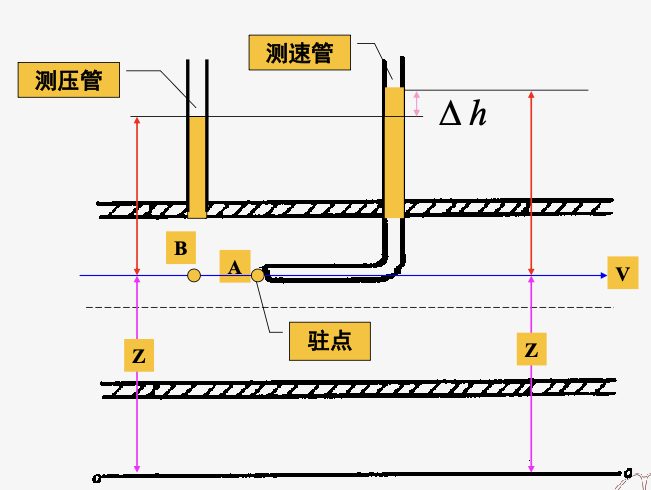
\includegraphics[width=\linewidth]{figures/3皮托管测速计.png}
\end{minipage}

\divider

\noindent
\begin{minipage}
    [t]{0.64\linewidth}
    \vspace{0pt}
    \raggedright
    \pt{文丘里流量计}\\
    以文丘里管水平轴线为基准面，对截面 $1$、$2$ 列伯努利方程：$\frac{p_1}{\rho g}+\frac{V_1^2}{2g}=\frac{p_2}{\rho g}+\frac{V_2^2}{2g}$\\
    由一维流动连续性方程 $V_1=\frac{A_2}{A_1}V_2$,$V_2=\sqrt{\frac{2(p_1-p_2)}{\rho[1-(A_2/A_1)^2]}}$
\end{minipage}
\hfill
\begin{minipage}
    [t]{0.35\linewidth}
    \vspace{0pt}
    \centering
    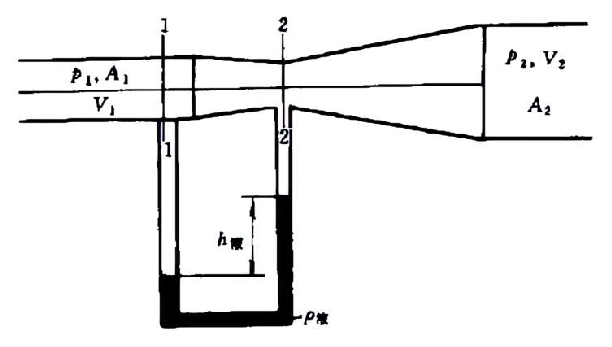
\includegraphics[width=\linewidth]{figures/3文丘里流量计.png}
\end{minipage}

$q_V=A_2V_2=\frac{\pi d_2^2}{4}\sqrt{\frac{2g(\rho_{\mathrm{液}}-\rho)h_{\mathrm{液}}}{\rho[1-(A_2/A_1)^2]}}$，实际体积流量 $q_{V,\mathrm{实}}=C_d q_V$，其中 $C_d$ 为流量系数，通过实验测定

\divider

%\subsection{定常流动的动量方程}

\pt{不可压缩流体动量方程}$\sum\vec{F}=\rho q_V(\beta_2\vec{V}_2-\beta_1\vec{V}_1)$

\divider

  \section{第四章\quad 黏性流体运动及其阻力计算}

%\subsection{黏性流体运动的两种状态}

雷诺实验说明黏性流体有两种基本流态：层流状态和紊流状态，中间可出现过渡状态。\pt{小流量}时，染色液体呈清晰细线，流体质点基本不混杂，对应\pt{层流}。\pt{中流量}时，染色线开始摆动、扩散，对应\pt{过渡状态}。\pt{大流量}时，染色液体迅速扩散并与主流混合，对应\pt{紊流}。

流速增加时：$v<v_c$ 为层流；$v=v_c \to v_c'$ 时由层流进入过渡状态；$v>v_c'$ 为紊流。
流速减小时：$v=v_c' \to v_c$ 时由紊流进入过渡状态；$v<v_c$ 又恢复层流。称 $v_c'$ 为上临界速度，$v_c$ 为下临界速度。$V_c \propto \mu/(\rho d)$ \\

雷诺实验\pt{结论}：当流速大于上临界流速时为紊流；小于下临界流速时为层流；介于两者之间时，流态可能是层流也可能是紊流，取决于初始状态和外界扰动。 \\
临界雷诺数定义为 $\mathrm{Re}_c=\frac{Vd_e}{\nu}$，其中 $\nu=\frac{mu}{\rho}$。下临界雷诺数 $\mathrm{Re}_c=2300$，是流态的判别标准，只取决于流体的过水断面形状，上临界雷诺数 $\mathrm{Re}_c'=\frac{V_c'd}{\nu}$ 极易受外界扰动影响，数值不稳定，实际意义不大。

当流体流动的雷诺数 $\mathrm{Re}<\mathrm{Re}_c$ 时，流动状态为层流；当 $\mathrm{Re}>\mathrm{Re}_c$ 时，流动状态为紊流；当 $\mathrm{Re}$ 介于 $\mathrm{Re}_c$ 和 $\mathrm{Re}_c'$ 之间时，流动状态极不稳定，任意微小扰动都会破坏稳定，变为紊流。\\

工程上认为 $\mathrm{Re}le 2300$ 时为层流，$\mathrm{Re}>2300$ 为紊流。

流体在任意形状截面的管道中流动时雷诺数的形式为 $\mathrm{Re}=\frac{Vd_e}{\nu}$ 其中 $d_e=\frac{4A}{\xi}$ 为当量直径，$x$ 为湿周，指在总流的有效截面上，流体与固体壁面的接触长度。

充满流体的圆管：$d_e=d$。
边长为 $a$ 的正方形管道：$d_e=a$。
高为 $h$、宽为 $b$ 的长方形管道：$d_e=\frac{2hb}{h+b}$。
圆环形管道：$d_e=d_2-d_1$。
管束流道：$d_e=4(S_1S_2-\pi d^2/4)/(\pi d)=4S_1S_2/(\pi d)-d$。

\pt{雷诺数的物理意义}:$\mathrm{Re}=\frac{\rho Vl}{\mu}=\frac{\rho V^2 l^2}{\mu Vl}=\frac{\text{惯性力}}{\text{粘性力}}$。当 $\mathrm{Re}$ 较小时，粘性力占主导，流动状态为层流；当 $\mathrm{Re}$ 较大时，惯性力占主导，流动状态为紊流。

\pt{层流}又称片流，指流体质点不相互混杂，作有序的成层流动。\pt{特点}：有序性；黏性占主要作用；遵循牛顿内摩擦定律；能量损失与流速一次方成正比；常发生在低流速、小 $\mathrm{Re}$ 情况。\\
\pt{紊流}又称湍流，指速度、压力等物理量在时间和空间中发生不规则脉动的流体运动。\pt{特点}：无序性、随机性、有旋性、混掺性；受黏性和紊动共同作用；水头损失与流速的 $1.75 \sim 2$ 次方成正比；常发生在高流速、大 $\mathrm{Re}$ 情况。

\divider

%\subsection{管内流动阻力的两种类型}

\pt{沿程阻力}：流体与管壁面以及流体层之间存在摩擦力，流体沿路程流动时受到摩擦阻滞。\pt{沿程损失}：流体在缓变流整个流程中，为克服沿程阻力而损失的能量。

使用\pt{达西-威斯巴赫公式}计算沿程水头损失 $h_f=\lambda \frac{l}{d}\frac{V^2}{2g}$，沿程压强损失 $\Delta p_f=\lambda \frac{l}{d}\rho\frac{V^2}{2}$。
其中 $\lambda$ 为沿程阻力系数，无量纲；$l$ 为管长；$d$ 为管径；$V$ 为有效截面平均流速。

\pt{局部阻力}：流体流经阀门、弯管、变截面等局部装置时，由碰撞、旋涡等造成的阻力。\pt{局部损失}：流体在状态急剧变化的急变流中，为克服局部阻力而损失的能量。

局部水头损失通式：$h_j=\zeta \frac{\nu^2}{2g}$，对应压力损失可记为 $\Delta p_j=\zeta \rho \frac{V^2}{2}$。$\zeta$ 为局部损失系数，无量纲，一般由实验测定。

总能量损失 $h_w=\sum h_f+\sum h_j$，$\Delta p_w=\rho g h_w=\sum \Delta p_f+\sum \Delta p_j$。能量损失的量纲为长度，工程中也称为水头损失。

\divider

%\subsection{圆管内层流流动}

\pt{层流流速分布}推导：将 $\tau = -\mu \frac{\mathrm{d}\mu}{\mathrm{d}r}$ 带入沿程损失 $f_f = \frac{2\tau}{r\rho g}l$ 得到 $\mathrm{d}u = -\frac{\Delta p_f}{2\mu l}r \mathrm{d}r$ 积分得到 $u = - \frac{\Delta p_f}{4\mu l}r^2+C$ 带入边界条件得到 $C = \frac{\Delta p_f}{4\mu l }{r_0}^2$，即 $u = \frac{\Delta p_f}{4\mu l}({r_0^2}-r^2)$，$u_\text{max}=\frac{\Delta p_f}{4\mu l}{r_0}^2$，$u = u_\text{max}\left(1-\frac{r^2}{{r_0}^2}\right)$

\pt{圆管内层流流量（哈根-泊肃叶公式）}$q_v =\frac{\Delta p_f \pi}{8\mu l}{r_0}^4$，\\\pt{平均流速}$V = \frac{\Delta p_f}{8\mu l}{r_0}^2$ 为最大流速的一半\\\pt{切应力}$\tau =\frac{\Delta p_f r}{2l}$，管壁上为 $\tau _0 =\frac{\Delta p_f r_0}{2l}$，则 $\tau = \tau_0\left(\frac{r}{r_0}\right)$

\pt{圆管内层流沿程损失}$h_f = \frac{32\mu l V}{\rho g d^2}=\lambda \frac{l}{d}\frac{V^2}{2g}$ 其中 $\lambda = \frac{64}{\mathrm{Re}}$\\

\pt{动能修正系数}$\alpha = \frac{1}{A}\iint_A\left(\frac{u}{V}\right)^3\,\mathrm{d}A=\frac{1}{\pi {r_0}^2}\int_{0}^{r_0} \left\{2\left[1-\left(\frac{r}{r_0}\right)^2\right]\right\}^3\times 2\pi r \, \mathrm{d}r = 2$

\divider

%\subsection{圆管内的紊流流动}

紊流是随机的三维非定常有旋流动，判据仍以雷诺数 $\mathrm{Re}$ 为基础。\pt{脉动现象}：流动参数随时间变化的现象。\pt{时均速度}：$\bar{u}=\frac{1}{t_1}\int_0^{t_1}u,\mathrm{d}t$。\pt{脉动速度}：$u'$。瞬时速度分解：$u=\bar{u}+u'$。同理，压力和密度也可写为：$p=\bar{p}+p'$，$\rho=\bar{\rho}+\rho'$。

\pt{紊流的速度分布}：靠近壁面处，速度按近似直线规律分布，属于黏性底层。靠近管轴中心处，速度按对数规律分布，属于紊流核心区。紊流核心区速度梯度较小，速度分布较均匀；管轴线处速度最大，因为紊流中质点脉动掺混强烈，动量交换明显。

\par\vspace{0.5pt}
{\centering
    \renewcommand{\arraystretch}{1.6}
    \resizebox{\linewidth}{!}{%
        \begin{tabular}{c|c|c|c|c|c}
            \hline
            $\boldsymbol{Re}$
             & $\mathbf{4.0\times10^3}$
             & $\mathbf{2.3\times10^4}$
             & $\mathbf{1.1\times10^5}$
             & $\mathbf{1.1\times10^6}$
             & $\mathbf{(2.0\sim3.2)\times10^6}$ \\
            \hline
            $\boldsymbol{V'/u_{\max}}$
             & $\mathbf{0.7912}$
             & $\mathbf{0.8073}$
             & $\mathbf{0.8167}$
             & $\mathbf{0.8497}$
             & $\mathbf{0.8658}$                 \\
            \hline
        \end{tabular}%
    }
    \par}

\pt{紊流结构分区}：黏性底层区，也称层流底层；层流向紊流的过渡区；充分发展紊流区，也称紊流核区。流速越高，$\mathrm{Re}$ 越大，层流底层越薄。
绝对粗糙度 $\Delta$：管壁粗糙凸出部分的平均高度。相对粗糙度：$\Delta/d$。

\pt{水力光滑管的紊流区} $\delta=\frac{58.3d}{\mathrm{Re}^{0.875}}$，适用于 $4\times 10^3<\mathrm{Re}<10^5$\\
\pt{一般的形式} $\delta=\frac{32.8d}{\mathrm{Re}\sqrt{\lambda}}$，适用于已知沿程阻力系数 $\lambda$ 时。

若黏性底层厚度 $\delta>\Delta$，粗糙凸起被黏性底层淹没，管道表现为水力光滑管。若 $\delta<\Delta$，粗糙凸起伸出黏性底层，管道表现为水力粗糙管。同一根管道在不同流速下，可能表现为光滑管，也可能表现为粗糙管。

\pt{紊流的切向应力}:摩擦切向应力：由流体黏性和相邻流层时均速度差引起$\tau_v=\mu\frac{\mathrm{d}u}{\mathrm{d}y}$。
附加切向应力：由横向脉动速度、质点掺混和动量交换引起 $\tau_t\propto \left(\frac{\mathrm{d}u}{\mathrm{d}y}\right)^2$。 紊流总切应力：$\tau=\tau_v+\tau_t$。接近管壁处，$\tau_v$ 起主要作用，$\tau_t$ 可略去。管道中心处，质点混杂强烈，$\tau_t$ 起主要作用，$\tau_v$ 可略去。管壁切应力：$\tau_0=\frac{\Delta p r_0}{2l}$。流管表面切应力：$\tau=\frac{\Delta p r}{2l}$。有效截面上的切应力分布：$\tau=\tau_0\frac{r}{r_0}$。层流与紊流虽然切应力沿半径都呈线性分布形式，但 $\tau_0$ 不同，所以分布斜率不同。在层流底层中，摩擦切应力占主要地位。

在紊流核心中附加切应力占主要地位紊流沿程损失仍采用达西-威斯巴赫形式：$h_f=\lambda\frac{l}{d}\frac{V^2}{2g}$。紊流计算的关键是确定沿程阻力系数 $\lambda$。紊流中 $\lambda=f(\mathrm{Re},\Delta/d)$，即同时与雷诺数和相对粗糙度有关。

\divider

%\subsection{圆管流动的沿程损失系数的确定}

\pt{尼古拉兹实验}：研究不同雷诺数和不同粗糙度下圆管沿程阻力系数 $\lambda$ 的变化规律。将黄沙筛分成由细到粗六种颗粒，分别粘贴在光滑管内壁上，形成不同人工粗糙度。采用三种不同管径：$25,\mathrm{mm}$、$50,\mathrm{mm}$、$100,\mathrm{mm}$。采用六种不同粗糙度，以通过改变流量改变 $\mathrm{Re}$。测出沿程损失 $h_f$，再由 $h_f=\lambda\frac{l}{d}\frac{V^2}{2g}$ 反求 $\lambda$。 $r/\Delta$ 表示，数值为 $15$、$30.6$、$60$、$126$、$252$、$507$。

\noindent
\begin{minipage}[t]{0.64\linewidth}
    \vspace{0pt}
    \raggedright
    $\MRN{1}$ 层流区：$\mathrm{Re}<2300$，有 $\lambda=\frac{64}{\mathrm{Re}}$。\\
    $\MRN{2}$  过渡区：$2300<\mathrm{Re}<4000$，情况复杂，无一定规律。\\
    $\MRN{3}$  紊流水力光滑管区： $4000<\mathrm{Re}<59.6(r/\Delta)^{8/7}$。满足布拉修斯公式，$\lambda = \frac{0.3164}{\mathrm{Re}^{0.25}}$。$10^5 <\mathrm{Re}<3\times 10^6$满足尼古拉兹经验公式 $\frac{1}{\sqrt{\lambda}}= 2.0\lg(\mathrm{Re}\sqrt{\lambda})-0.8$\\
\end{minipage}
\hfill
\begin{minipage}[t]{0.35\linewidth}
    \vspace{0pt}
    \centering
    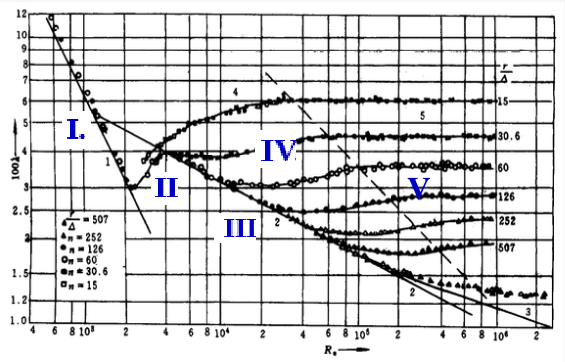
\includegraphics[width=\linewidth]{figures/4尼古拉兹实验曲线图.png}
\end{minipage}

$\MRN{4}$ 紊流水力粗糙管过渡区：$59.6(r/\Delta)^{8/7}<\mathrm{Re}<4160(r/\Delta)^{0.85}$。可使用洛巴耶夫公式 $$\lambda=1.42[\lg(\mathrm{Re}d/\Delta)]^{-2}=1.42[\lg(1.273q_V/(\nu\Delta))]^{-2}$$ 或者科尔布鲁克公式 $\frac{1}{\sqrt{\lambda}}=-2\lg\left(\frac{2.51}{\mathrm{Re}\sqrt{\lambda}}+\frac{\Delta/d}{3.7}\right)$ \\
$\MRN{5}$ 紊流水力粗糙管平方阻力区：$\mathrm{Re}>4160(r/\Delta)^{0.85}$，满足尼古拉兹经验公式 $\frac{1}{\sqrt{\lambda}}=2\lg\frac{d}{2\Delta}+1.74$

实验意义：紊流复杂，管壁粗糙度会影响 $\lambda$，无法像层流那样完全由理论推出。需要通过实验测定并归纳出经验公式。尼古拉兹实验是系统性强、参数范围广的代表性实验。实验局限：实验采用人工粗糙度，与工业管道自然粗糙度差异较大，不能直接完全套用。

\noindent
\begin{minipage}[t]{0.48\linewidth}
    \vspace{0pt}
    \raggedright
    \pt{莫迪图}\\
    适用范围为 $600<\mathrm{Re}<10^8$ 用图时通常根据 $ \mathrm{Re} $ 和 $ \Delta/d $ 查取 $ \lambda $。与尼古拉兹曲线相比，莫迪图更适合工程管道实际计算
\end{minipage}
\hfill
\begin{minipage}[t]{0.48\linewidth}
    \vspace{0pt}
    \centering
    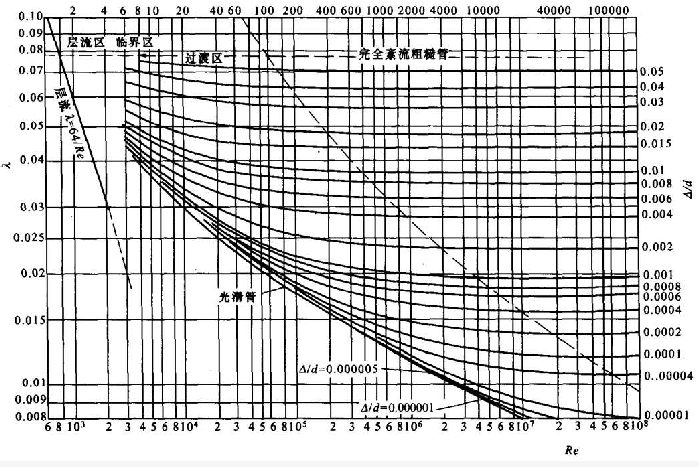
\includegraphics[width=\linewidth]{figures/4莫迪图.png}
\end{minipage}

\divider

%\subsection{局部损失计算}

局部损失产生位置：阀门、弯管、突然扩大、突然缩小等管件处。流通截面或流动方向急剧变化，引起速度场迅速改变，增加流体间摩擦、碰撞并形成旋涡，从而产生局部损失

$h_j = \frac{({V_1}^2-{V_2}^2)}{2g}=\frac{V_1^2}{2g}\left(1-\frac{A_1}{A_2}\right)^2=\frac{V_2^2}{2g}\left(\frac{A_2}{A_1}-1\right)^2$，$\zeta_1=\left(1-\frac{A_1}{A_2}\right)^2$，$\zeta_2=\left(\frac{A_2}{A_1}-1\right)^2$，则局部损失可写成 $h_j=\zeta_1\frac{V_1^2}{2g}=\zeta_2\frac{V_2^2}{2g}$。\\

\par\vspace{0.5pt}
{\centering
    \renewcommand{\arraystretch}{1.45}
    \resizebox{\linewidth}{!}{%
        \begin{tabular}{c|c|c|c|c|c|c|c|c|c|c|c}
            \hline
            $\frac{A_1}{A_2}=\left(\frac{d_1}{d_2}\right)^2$
             & $\mathbf{0}$
             & $\mathbf{0.1}$
             & $\mathbf{0.2}$
             & $\mathbf{0.3}$
             & $\mathbf{0.4}$
             & $\mathbf{0.5}$
             & $\mathbf{0.6}$
             & $\mathbf{0.7}$
             & $\mathbf{0.8}$
             & $\mathbf{0.9}$
             & $\mathbf{1.0}$ \\
            \hline
            $\zeta_1$
             & $1.0$
             & $0.81$
             & $0.64$
             & $0.5$
             & $0.36$
             & $0.25$
             & $0.16$
             & $0.09$
             & $0.04$
             & $0.01$
             & $0$            \\
            \hline
            $\zeta_2$
             & $\infty$
             & $81$
             & $16$
             & $5.44$
             & $2.25$
             & $1.0$
             & $0.444$
             & $0.184$
             & $0.0625$
             & $0.0123$
             & $0$            \\
            \hline
        \end{tabular}%
    }
    \par}

突然扩大 $A_2\gg A_1$，$\zeta_1 \approx 1,\zeta_2 \approx \infty$，突然缩小有经验公式 $\zeta_2 =0.5 \left(1-\frac{A_2}{A_1}\right)$ $A_1\gg A_2$，$\zeta_2 \approx 0.5$。\\

\divider

%\subsection{管道水力计算}

\pt{管道系统分类}
\begin{itemize}
    \item \pt{按照能量损失大小分类}：长管：局部阻力在总阻力中的比例不足 $5\%$ 的管道系统，称为水力长管，计算时只考虑沿程损失；短管：水力计算中需要同时考虑沿程损失和局部损失的管道系统。
    \item \pt{按照管道系统结构}：简单管道：管径和粗糙度均相同的一根或数根管子串联而成；复杂管道：包括串联管道、并联管道、枝状管道、网状管道。
\end{itemize}

管道系统分类类似电路系统，水力计算类似电路计算。将管道中的流量比作电流，压降比作电压降\\

\pt{串联管道}：串联管道中各段的流量相等，对于不可压缩流体 $q*{V1}=q*{V2}=q_{V3}=\cdots=\mathrm{const}$，$V_1A_1=V_2A_2=V_3A_3=\cdots=\mathrm{const}$。总能量损失是各段管道中的能量损失之和 $h_w = h_{w1}+h_{w2}+h_{w3}+\cdots$，若各管段的管径相同，称为简单管道，则各管段的平均流速也相等

\pt{并联管道}：对于不可压缩流体 $q_V = q_{V1}+q_{V2}+q_{V3}+\cdots$，两点之间的能量损失相同，为这两节点之间的压头差 $h_{W1}=h_{w2}=h_{w3}=h_{w(a-b)}$

\pt{基本公式}：\\
\pt{连续性方程}：$q_m=\rho_1gV_1A_1=\rho_2gV_2A_2=\mathrm{const}$ 或者 $q_V = V_1A_1=V_2A_2 =\mathrm{const}$\\
\pt{伯努利方程}:$z_1+\frac{p_1}{\rho g}+\frac{{V_1}^2}{2g}=z_2+ \frac{p_2}{\rho g}+h_2$\\
\pt{能量损失}:$h_w = \sum h_f +\sum h_j$, $h_f=\lambda \frac{l}{d}\frac{V^2}{2g}$,$h_j=\zeta \frac{V^2}{2g}$

\divider

  \section{第五章 \quad 传热分析基础}

%\subsection{传热学概论}

传热学是研究在温差作用下热量传递规律的一门学科

主要研究：热量传递机理：热能如何通过导热、对流、辐射传递。热量传递规律：传递热量与温差之间的定量关系，以及温度分布的数学描述。热量传递规律的测试方法：通过实验测试获得传热过程规律

传热学研究的三类问题：强化传热、传热削弱和温度控制。

传热学的热阻思想：$\Phi =\lambda A\frac{\Delta t}{\delta}=\frac{\Delta t}{\delta / (\lambda A)}$ 我们称 $\Delta t$ 为温压，$\delta . (\lambda/A)$ 为热阻 $R_\lambda$，热阻可以串联、并联等

三种基本传热方式：热传导、热对流和热辐射

\pt{热传导}是温度不同的物体各部分之间，或温度不同且直接接触的两物体之间，依靠分子、原子、自由电子等微观粒子热运动进行的热量传递。导热是物体的固有本质，只要存在温差，固体、液体、气体中都可以发生导热。热传导满足\pt{傅里叶定律}：$q=\frac{\Phi}{A}=-\lambda \frac{\mathrm{d}t}{\mathrm{d}x}$。$\Phi$ 为热流量，单位 $\mathrm{W}$；$q$ 为热流密度，单位 $\mathrm{W}/\mathrm{m}^2$；$\lambda$ 为导热系数，单位 $\mathrm{W}/(\mathrm{m}\cdot\mathrm{K})$

\pt{热对流}：流体各部分之间发生相对位移时，冷热流体相互掺混所引起的热量传递过程。只能发生在流体中；是流体宏观运动引起的能量传递与流体分子导热共同作用的结果。对流换热是流体流过温度不同的固体壁面时，流体与固体壁面之间的热量传递过程。热对流满足\pt{牛顿冷却公式} $t_w>t_f,q=\frac{\Phi}{A}=h(t_w-t_f)$，$t_f>t_w,q=\frac{\Phi}{A}=h(t_f-t_w)$。其中 $t_w$ 是壁面温度，$t_f$ 是流体温度，$A$ 为与流体接触的壁面面积，$h$ 是对流换热系数，单位 $\mathrm{W}/(\mathrm{m}^2\cdot\mathrm{K})$。$h$ 表征对流换热强弱，是过程量，与流体种类、表面形状、流体速度等因素有关

\pt{热辐射}：物体通过电磁波传递能量；热辐射是物体由于热的原因向外发出的辐射；辐射传热是物体之间以辐射形式进行的热量交换。黑体是能吸收投入到其表面上全部热辐射能的理想物体，其辐射能力只与温度有关。黑体辐射满足\pt{斯特藩-玻尔兹曼定律}：$E=\sigma t^4$，其中 $\sigma$ 是斯特藩-玻尔兹曼常数，数值为 $5.67\times 10^{-8}\mathrm{W}/(\mathrm{m}^2\cdot\mathrm{K}^4)$；实际物体对外辐射热流量的计算式为 $\Phi =\varepsilon A \sigma T^4$。$\varepsilon$ 为发射率/黑度，$\varepsilon\le 1$，与物体种类、表面状况、温度有关。

实际热量传递常不是单一方式：多个环节可以串联，同一环节中也可能有多种方式同时作用。\pt{传热过程}：热量由壁面一侧流体通过壁面传到另一侧流体中的过程，典型如换热器中热流体向冷流体传热.\pt{传热方程式} $\Phi=kA(t_{f1}-t_{f2})$，$k$ 为传热系数，表示整个传热过程强弱，单位 $\mathrm{W}/(\mathrm{m}^2\cdot\mathrm{K})$；$k$ 与组成过程的 $h_1$、$h_2$ 等有关。

\pt{流动传热学和工程热力学的关系}： 传热学与工程热力学都属于热学范畴；热力学第一定律是研究一切热传递现象的基本依据。两种介质分界面上的能量平衡可写为 $q_0^+=q_0^-$，本质是热力学第一定律的应用。热力学研究平衡态，更关心能量总量；传热学研究非平衡态，更关心热量传递速率，例如 $q$ 的单位为 $\mathrm{J}/(\mathrm{m}^2\cdot\mathrm{s})=\mathrm{W}/\mathrm{m}^2$。

对流换热与流体流动密不可分，流体力学是传热学的先修基础；流体力学通常研究等温流动和阻力，传热学研究有温差流动中的热量交换。

传热学的研究方法：实验研究：从传热学诞生至今一直是基本研究方法，依靠实验测定传热规律。数学理论分析：对物理过程作合理简化假设，建立数学描述，再用数学方法求解析解。计算机数值求解：把偏微分方程和边界条件在空间代表点上离散为代数方程组，再近似求解。

\divider

%\subsection{传热分析基本概念}

\pt{温度场}：各个时刻物体中各点温度值所组成的集合。按照温度场随空间与时间的变化特性，可以分为

\pt{稳态温度场} $t=f(\vec{r})$ 和 \pt{非稳态温度场} $t=f(\vec{r},t)$。按照维数可以分为 \pt{一维温度场} $t=f(x)$、\pt{二维温度场} $t=f(x,y)$ 和 \pt{三维温度场} $t=f(x,y,z)$（以及是否带时间）\\

\pt{等温线（面）}同一瞬间温度相等的各点连成的线或者面被称为等温线或者等温面。等温线或者等温面不能相交，因为同一点不可能同时有两个温度；只能在物体边界中断或完全封闭。局部热流密度与等温线垂直。若相邻等温线温差相同，等温线越密，局部热流密度越大。若等温线处处垂直于某界面，则该界面为绝热面；绝热边界满足 $\partial t/\partial n=0$。

\pt{温度梯度}：某点所在等温线与相邻等温线之间的温差与其法线距离之比取极限，是指向温度升高方向的向量。$\operatorname{grad}(t)=\lim_{n\to \infty}\left(\frac{\Delta t}{\Delta n}\right)=\frac{\partial t}{\partial n}\vec{n}=\frac{\partial t}{\partial x}\vec{i}+\frac{\partial t}{\partial y}\vec{j}+\frac{\partial t}{\partial n}\vec{n}$

\divider
  \section{第六章 \quad 导热的基础与理论计算}

\pt{导热机理}气体：主要来自分子热运动，$t$ 升高时 $\lambda$ 增大。导电固体：主要来自自由电子运动。非导电固体：主要来自晶格振动，量子化后称为声子。液体：来自分子热运动及晶格振动。

傅里叶发现单位时间内通过给定截面的热量，正比于垂直该截面方向上的温度变化率和截面面积，方向与温度梯度相反。

数学描述为 $\vec{q}=\frac{\vec{\Phi}}{A}-\lambda \operatorname{grad}(t)=-\lambda \frac{\partial t}{\partial n}\vec{n}$ 实验定律，常规尺度问题普遍适用：变物性，内热源，非稳态，固、液、气。负号含义：热量传递方向指向温度降低方向，与温度升高方向相反。热流密度矢量与等温线或等温面垂直，且方向与温度梯度相反；其走向可用热流线表示。

\pt{导热系数}$\lambda =\frac{\vert \vec{q} \vert}{\vert \operatorname{grad}t\vert}$ 物理意义：数值上等于单位温度梯度作用下物体内产生的热流密度的模，是标量，单位为 $\mathrm{W/(m\cdot K)}$。表征物体导热本领大小。与物质种类及热力状态有关，如温度、气体压力等；与宏观物体几何形状无关。导热系数数量级：气体最低，建筑与绝热材料较低，液体居中，非金属固体更高，金属和非金属晶体可很高。常用大小顺序：$\lambda_{\mathrm{金属}}>\lambda_{\mathrm{非金属}}$，$\lambda_{\mathrm{固相}}>\lambda_{\mathrm{液相}}>\lambda_{\mathrm{气相}}$。常温约 $20^\circ\mathrm{C}$ 示例：纯铜 $\lambda=399,\mathrm{W/(m\cdot K)}$，纯钛 $\lambda=36.7,\mathrm{W/(m\cdot K)}$，水 $\lambda=0.599,\mathrm{W/(m\cdot K)}$，空气 $\lambda=0.0259,\mathrm{W/(m\cdot K)}$。温度范围不宽时，工程材料导热系数可近似写成线性函数：$\lambda=\lambda_0(1+bt)$。本课程只讨论各向同性材料，认为材料的 $\lambda$ 及其随温度变化关系已知。

\divider

%\subsection{导热问题的数学描述微分方程及其定解条件}

任意三维的非稳态导热体，且物体内有内热源，假设为各向同性连续介质，导热系数、比热容和密度均已知，内热源均匀分布，强度为 $\dot{\Phi}$，单位 $\mathrm{W/m^3}$，且导热体与外界没有功的交换。

\pt{单位时间导入的静热量}为 $\Phi_c = \left[\frac{\partial }{\partial x}\left(\lambda \frac{\partial t}{\partial x}\right)+\frac{\partial }{\partial y}\left(\lambda \frac{\partial t}{\partial y}\right)+\frac{\partial }{\partial z}\left(\lambda \frac{\partial t}{\partial z}\right)\right]\,\mathrm{d}x\mathrm{d}y\mathrm{d}z$\\
\pt{单位时间内微元体内热源生成的热量} $\Phi_V = \dot{\Phi}\, \mathrm{d}x\mathrm{d}y\mathrm{d}z$\\
\pt{单位时间内微元体热力学能增量} $\Delta U =\rho c \frac{\partial t}{\partial \tau}\cdot \mathrm{d}x\mathrm{d}y\mathrm{d}z$\\
由能量守恒，得到导热微分方程的基本形式

$\rho c\frac{\partial t}{\partial\tau}=\frac{\partial}{\partial x}(\lambda\frac{\partial t}{\partial x})+\frac{\partial}{\partial y}(\lambda\frac{\partial t}{\partial y})+\frac{\partial}{\partial z}(\lambda\frac{\partial t}{\partial z})+\dot{\Phi}$

$\rho c\partial t/\partial\tau$ 为非稳态项；三个空间导热项为导热项或扩散项；$\dot{\Phi}$ 为内热源项（按课件上排版不下，哎）

$\lambda =\mathrm{const}$ 时 $\frac{\partial t}{\partial\tau}=\frac{\lambda}{\rho c}\left(\frac{\partial^2t}{\partial x^2}+\frac{\partial^2t}{\partial y^2}+\frac{\partial^2t}{\partial z^2}\right)+\frac{\dot{\Phi}}{\rho c}$，令 $a=\frac{\lambda}{\rho c}$ 单位 $\mathrm{m^2/s}$，是物性参数，则 $\frac{\partial t}{\partial\tau}=a\left(\frac{\partial^2t}{\partial x^2}+\frac{\partial^2t}{\partial y^2}+\frac{\partial^2t}{\partial z^2}\right)+\frac{\dot{\boldsymbol{\Phi}}}{\rho c}$

$\lambda=\mathrm{const}$ 且无内热源时 $\frac{\partial t}{\partial \tau}=a\nabla^2 t$

$\lambda = \mathrm{const}$ 且稳态时 $\nabla^2 t = -\frac{\dot{\Phi}}{\lambda}$ 称为 Poisson 方程

$\lambda = \mathrm{const}$，稳态，且无内热源时 $\nabla^2 t = 0$ 称为 Laplace 方程

$\lambda = \mathrm{const}$，稳态，一维时 $\frac{\mathrm{d}^2 t}{\mathrm{d}x^2}+\frac{\dot{\Phi}}{\lambda}=0$

$\lambda = \mathrm{const}$，稳态，无内热源且一维时 $\frac{\mathrm{d}^2 t}{\mathrm{d}x^2}=0$

柱坐标系中 $\rho c \frac{\partial t}{\partial \tau} =\frac{1}{r} \frac{\partial}{\partial r}\left(r \lambda \frac{\partial t}{\partial r}\right)+\frac{1}{r^2} \frac{\partial}{\partial \theta}\left(\lambda \frac{\partial t}{\partial \theta}\right)+\frac{\partial}{\partial z}\left(\lambda \frac{\partial t}{\partial z}\right)+\dot{\Phi}$

球坐标系中 $\rho c \frac{\partial t}{\partial \tau}=\frac{1}{r^2} \frac{\partial}{\partial r}\left(r^2 \lambda \frac{\partial t}{\partial r}\right)+\frac{1}{r^2 \sin \theta} \frac{\partial}{\partial \theta}\left(\sin \theta \lambda \frac{\partial t}{\partial \theta}\right)+\frac{1}{r^2 \sin^2 \theta} \frac{\partial}{\partial \varphi}\left(\lambda \frac{\partial t}{\partial \varphi}\right)+\dot{\Phi}$

\pt{定解条件}：分为初值条件和边界条件

\pt{初值条件}给定初始时刻的温度分布 $t = f(x,y,z) \quad \text{at} \quad \tau = 0$\\
\pt{边界条件}有三类

\begin{itemize}
    \item \pt{第一类边界条件，Dirichlet 条件}边界上的温度分布 $t_w = f(\tau)$
    \item \pt{第二类边界条件，Neumann 条件}边界上的热流密度分布 $-\lambda \frac{\partial t}{\partial n}\vert _w = f(\tau)=q_w$
    \item \pt{第三类边界条件，Robin 条件}给定边界上的热流密度与边界温度的关系 $-\lambda \frac{\partial t}{\partial n}\vert _w = h(t_w-t_f)$
    \item \pt{辐射边界条件} $-\lambda\left.\frac{\partial T}{\partial n}\right|_w=\varepsilon\sigma(T_w^4-T_e^4)$
    \item \pt{界面连续条件} $\left(\lambda\frac{\partial t}{\partial n}\right)_1=\left(\lambda\frac{\partial t}{\partial n}\right)_2$
\end{itemize}

Fourier 定律及导热微分方程不适用于以下情形：导热物体温度接近绝对零度时，即温度效应显著；过程作用时间极短，接近材料本身固有时间尺度时，即时间效应显著；过程空间尺度极小，接近微观粒子平均自由程时，即尺度效应显著。上述导热过程称为非傅里叶导热，即 $\mathrm{Non\text{-}Fourier\ heat\ conduction}$。

\divider

%\subsection{典型一维稳态导热问题的分析解}

\pt{单层平壁导热问题分析解}

\pt{稳态无内热源常导热系数第一类边界条件}

$\left\{
    \begin{aligned}
         & \frac{\mathrm{d}^2 t}{\mathrm{d}x^2}=0 \\
         & x=0,t=t_1                              \\
         & x=\delta,t=t_2
    \end{aligned}
    \right.
$ 解得 $\left\{
    \begin{aligned}
         & \frac{\mathrm{d}^2 t}{\mathrm{d}x^2}=0 \\
         & x=0-,t=t_1                             \\
         & x=\delta,t=t_2
    \end{aligned}
    \right.$ $\left\{
    \begin{aligned}
         & \text{单位面积热阻} r=\frac{\delta }{\lambda} \text{单位} \mathrm{m^2\cdot K/W} \\
         & \text{总面积热阻} R=\frac{\delta}{\lambda A} \text{单位} \mathrm{K/W}          \\
    \end{aligned}
    \right.$

\pt{稳态无内热源常导热系数第一类边界条件}

$\left\{
    \begin{aligned}
         & \frac{\mathrm{d}}{\mathrm{d}x}\left(\lambda \frac{\mathrm{d}t}{\mathrm{d}x}\right)= 0 \\
         & x=0,t=t_1                                                                             \\
         & x=\delta,t=t_2                                                                        \\
         & \lambda = \lambda_0(1+b t)
    \end{aligned}
    \right.$ 解得 $\left\{
    \begin{aligned}
         & q = \frac{\bar{\lambda}(t_2-t_1)}{\delta}     \\
         & \Phi = \frac{\bar{\lambda}A(t_2-t_1)}{\delta}
    \end{aligned}
    \right.$

\pt{多层平壁导热的分析解}：认为其热阻为各层热阻之和，则对于 $n$ 层平壁 $q = \frac{t_1-t_{n+1}}{\sum_{i=1}^n (\delta_i/\lambda_i)}$

\pt{接触热阻}：两个名义上平整的固体表面相互接触时，实际固体-固体接触只发生在离散接触面上。不贴合部分存在空隙，空气导热系数小，会产生额外热阻，称为接触热阻。接触热阻通常由实验测定。减小接触热阻的方法表面加工得更光滑，保持表面干净，加导热油、碳粉、金属粉、导热硅胶等填充材料。多层导热题若题目说明“忽略接触热阻”，就只串联材料热阻；若考虑接触热阻，应把接触热阻作为额外热阻加入总热阻。

\divider

\pt{通过单层圆筒壁的导热}

\pt{稳态无内热源常导热系数第一类边界条件}

$\left\{
    \begin{aligned}
         & \frac{\mathrm{d}}{\mathrm{d}r}\left(r  \frac{\mathrm{d}t}{\mathrm{d}r}\right)=0 \\
         & r=r_1,t=t_1                                                                     \\
         & r=r_2,t=t_2
    \end{aligned}
    \right.$，解得 $\left\{
    \begin{aligned}
         & t = t_1 + \frac{t_2-t_1}{\ln(r_2/r_1)}\ln\left(\frac{r}{r_1}\right)        \\
         & \Phi=\frac{t_1-t_2}{\frac{1}{2\pi\lambda l}\ln(r_2/r_1)}=\frac{t_1-t_2}{R}
    \end{aligned}
    \right.$

多层则依旧看作热阻串联，$\Phi = \frac{t_1-t_{n+1}}{\sum_{i=1}^n (\frac{1}{2\pi\lambda_i l}\ln(r_{i+1}/r_i))}$

\divider

\pt{通过球壳壁的导热}

$\left\{
    \begin{aligned}
         & \frac{\mathrm{d}}{\mathrm{d}r}\left(r^2  \frac{\mathrm{d}t}{\mathrm{d}r}\right)=0 \\
         & r=r_1,t=t_1                                                                       \\
         & r=r_2,t=t_2
    \end{aligned}
    \right.$，解得 $\left\{
    \begin{aligned}
         & t = t_1 + \frac{t_2-t_1}{1/r_1-1/r_2}\left(\frac{1}{r}-\frac{1}{r_1}\right)                         \\
         & \Phi =\frac{4\pi\lambda\left(t_1-t_2\right)}{1/r_1-1/r_2}=\frac{t_1-t_2}{(1/r_1-1/r_2)/4\pi\lambda} \\
         & R=\frac{1}{4\pi\lambda}(1/r_1-1/r_2)
    \end{aligned}
    \right.$

\divider

\pt{第二三类边界条件一维导热问题}

\pt{第二类边界条件}

$\left\{
    \begin{aligned}
         & \frac{\mathrm{d}^2 t}{\mathrm{d}x^2}=0                       \\
         & x=0,t=t_1                                                    \\
         & x=\delta,-\lambda \frac{\mathrm{d}t}{\mathrm{d}x}\vert = q_w
    \end{aligned}
    \right.$，解得 $t = -\frac{q_w}{\lambda}x+t_1$

\pt{第三类边界条件}（壁温 $t_2$ 未知，热流温度 $t_f$ 已知）

$\left\{
    \begin{aligned}
         & \frac{\mathrm{d}^2 t}{\mathrm{d}x^2}=0                           \\
         & x=0, t=t_1                                                       \\
         & x=\delta , -\lambda \frac{\mathrm{d}t}{\mathrm{d}x} = h(t_2-t_f)
    \end{aligned}
    \right.$ 解得 $
    \begin{aligned}
        t_2 & =\frac{\lambda t_1+h\delta t_f}{\lambda+h\delta} \\
        t   & =\frac{h(t_2-t_f)}{\lambda}x+t_1                 \\
            & =-\frac{h(t_1-t_f)}{\lambda+h\delta}x+t_1
    \end{aligned}
$

可以使用热阻思想，将两个表面的对流传热热阻叠加进去，将温差改为两个流体的温差 $q = \frac{t_{f1}-t_{f2}}{\frac{1}{h}+\sum_{i=1}^{n}\frac{\delta_i}{\lambda_i}+\frac{1}{h_2}}$

\divider

%\subsection{非稳态导热的基本概念与数学描述}

\pt{非稳态导热分类}：周期性非稳态导热：物体中各点温度及热流密度随时间周期性变化，例如太阳辐照引起地球温度变化。非周期性非稳态导热：物体温度随时间逐渐趋于恒定值，例如动力机械从启动到稳定运行；本章主要研究这一类。温度变化率范围很宽，可从 $10^{-4},\mathrm{K/s}$ 到 $10^{12},\mathrm{K/s}$；极高速情形下 Fourier 定律可能不再适用。

\pt{非稳态导热特点}：热扰动从界面传到一定距离需要时间。同一时刻，不同截面上的导热量不同，即一般有 $\Phi_1\ne \Phi_2$温度分布有两个阶段：非正规状况阶段：温度分布主要受初始温度分布影响.正规状况阶段：初始温度分布影响逐渐消失，不同时刻温度分布主要取决于边界条件及物性。

导热微分方程统一形式 $\rho c \frac{\partial t}{\partial \tau}=\lambda \operatorname{div}(\operatorname{grad}t)+\dot{\Phi}$ 或者 $\frac{\partial t}{\partial \tau}=\lambda\nabla^2t+\frac{\dot{\Phi}}{\rho c}$ 主要讨论第三类边界条件

毕渥数定义：对厚为 $2\delta$ 的平板，$\mathrm{Bi}=\frac{h\delta}{\lambda}=\frac{\delta/\lambda}{1/h}$。物理意义：$\mathrm{Bi}=\frac{\text{物体内部导热热阻}}{\text{物体表面对流传热热阻}}$。$\delta$ 是平板半厚，属于特征尺度。

$\mathrm{Bi}\to\infty$：表面换热极强，$h\to\infty$，对流热阻趋近 0，表面温度几乎立即降到 $t_\infty$，第 $\MRN{3}$  类边界条件趋向第 $\MRN{1}$  类边界条件。
$\mathrm{Bi}\to 0$：物体导热系数很大，内部导热热阻趋近 $0$，任意时刻物体内部温度近似均匀；这是集中参数法的基础。
$0<\mathrm{Bi}<\infty$：对流热阻与导热热阻同量级，情况介于上述两者之间。

像 $\mathrm{Bi}$ 这样表征物理过程特征的无量纲数称为特征数或准则数。学习特征数时要掌握定义、特征尺度取法和物理意义。

\divider

%\subsection{集中参数法}

\pt{集中参数法}基本思想：当 $\mathrm{Bi}\to 0$ 时，物体内部导热热阻远小于表面对流热阻，物体内部任意时刻温度趋于一致。温度只随时间变化，不随空间变化：$t=f(\tau)$。这种零维处理方法称为集中参数法。只要物体内部任意时刻温度基本均匀，无论形状、加热或冷却，都可用集中参数法。

\pt{数学描述}：$\frac{\mathrm{d}t}{\mathrm{d}\tau}=\frac{\Phi}{\rho c}$，能量微分方程化为 $\rho Vc\frac{\mathrm{d}t}{\mathrm{d}\tau}=-Ah(t-t_\infty)$，解得 $\frac{\theta}{\theta_0}=\frac{t-t_\infty}{t_0-t_\infty}=\exp\left(-\frac{hA}{\rho Vc}\tau\right)$，指数项可改写为 $\frac{hA}{\rho Vc}\tau=\frac{h(V/A)}{\lambda}\frac{a\tau}{(V/A)^2}=\mathrm{Bi}_V\mathrm{Fo}_V$ $\mathrm{Bi}_V$ 是以 $l_c=V/A$ 为特征长度的毕渥数。$\mathrm{Fo}_V$ 是以 $l_c=V/A$ 为特征长度的傅里叶数。

\pt{傅里叶数}：定义：$\mathrm{Fo}=\frac{a\tau}{l_c^2}=\frac{\tau}{l_c^2/a}$。物理意义：$\mathrm{Fo}$ 是表征非稳态过程进行深度的无量纲时间。$\mathrm{Fo}$ 越大，热扰动越深入地传播到物体内部，物体内各点温度越接近周围介质温度。

\pt{非稳态导热量}：瞬时热流量：$\Phi(\tau)=-\rho cV\frac{\mathrm{d}t}{\mathrm{d}\tau}=hA(t-t_\infty)$。从 $0$ 到 $\tau$ 的总换热量：$Q_{0-\tau}=\int_0^\tau\Phi(\tau)\mathrm{d}\tau$。也可由内能变化得：$Q_{0-\tau}=\rho Vc(t_0-t)$。写成指数形式：$Q_{0-\tau}=\theta_0\rho Vc\left[1-\exp\left(-\frac{hA}{\rho Vc}\tau\right)\right]$。

\pt{时间常数}：定义：令 $\frac{hA}{\rho Vc}\tau=1$ 的时间为时间常数 $\tau_c$。$\tau_c=\frac{\rho Vc}{hA}$。当 $\tau=\tau_c$ 时，$\frac{\theta}{\theta_0}=e^{-1}=0.368$，过程完成 $63.2\%$。$\tau_c$ 越小，对温度变化响应越快。动态测温中，时间常数越小，越能正确反映被测温度变化。

\pt{集中参数法适用范围}：一般要求 $\mathrm{Bi}=\frac{hl}{\lambda}\le 0.1$，此时物体中各点过余温度差别小于等于 $5\%$。若直接取几何特征长度：厚度 $2\delta$ 平板：$\mathrm{Bi}=\frac{h\delta}{\lambda}\le 0.1$。半径 $R$ 圆柱：$\mathrm{Bi}=\frac{hR}{\lambda}\le 0.1$。半径 $R$ 球：$\mathrm{Bi}=\frac{hR}{\lambda}\le 0.1$。若取 $l_c=V/A$：无限大平板：$l_c=\delta$，$\mathrm{Bi}=\frac{h\delta}{\lambda}\le 0.1$。无限长圆柱：$l_c=0.5R$，$\mathrm{Bi}=\frac{hR}{2\lambda}\le 0.05$。圆球：$l_c=R/3$，$\mathrm{Bi}=\frac{hR}{3\lambda}\le 0.033$。课件强调：零维问题中特征尺度计算很关键，要分析清楚发生导热的体积 $V$ 和换热面积 $A$。

\divider

%\subsection{典型一维非稳态导热问题的分析解}

当非稳态导热问题不满足集中参数法条件，或研究目的本身需要确定物体内部温度差异时不使用集中参数法。

{\centering
\renewcommand{\arraystretch}{1.85}
\resizebox{\linewidth}{!}{%
    \begin{tabular}{c|c|c|c|c|c}
        \hline
        \textbf{形状}
         & \textbf{无量纲温度分析解}
         & $\boldsymbol{\mu_n}$ \textbf{是下列超越方程的根}
         & $\boldsymbol{\eta}$
         & $\boldsymbol{\mathrm{Fo}}$
         & $\boldsymbol{\mathrm{Bi}}$              \\
        \hline

        \textbf{平板}
         &
        $\begin{aligned}
                 \frac{\theta(\eta,\tau)}{\theta_0}
                  & = \sum_{n=1}^{\infty} C_n
                 \exp(-\mu_n^2 \mathrm{Fo})\cos(\mu_n\eta) \\
                 C_n
                  & = \frac{2\sin(\mu_n)}
                 {\mu_n+\sin(\mu_n)\cos(\mu_n)}
             \end{aligned}$
         &
        $\tan(\mu_n)=\frac{\mathrm{Bi}}{\mu_n},\ n=1,2,\cdots$
         &
        $\frac{x}{\delta}$
         &
        $\frac{a\tau}{\delta^2}$
         &
        $\frac{h\delta}{\lambda}$                  \\
        \hline

        \textbf{圆柱}
         &
        $\begin{aligned}
                 \frac{\theta(\eta,\tau)}{\theta_0}
                  & = \sum_{n=1}^{\infty} C_n
                 \exp(-\mu_n^2 \mathrm{Fo})J_0(\mu_n\eta) \\
                 C_n
                  & = \frac{2}{\mu_n}
                 \frac{J_1(\mu_n)}
                 {J_0^2(\mu_n)+J_1^2(\mu_n)}
             \end{aligned}$
         &
        $\mu_n\frac{J_1(\mu_n)}{J_0(\mu_n)}=\mathrm{Bi},\ n=1,2,\cdots$
         &
        $\frac{r}{R}$
         &
        $\frac{a\tau}{R^2}$
         &
        $\frac{hR}{\lambda}$                       \\
        \hline

        \textbf{球}
         &
        $\begin{aligned}
                 \frac{\theta(\eta,\tau)}{\theta_0}
                  & = \sum_{n=1}^{\infty} C_n
                 \exp(-\mu_n^2 \mathrm{Fo})
                 \frac{\sin(\mu_n\eta)}{\mu_n\eta}           \\
                 C_n
                  & = \frac{2[\sin(\mu_n)-\mu_n\cos(\mu_n)]}
                 {\mu_n-\sin(\mu_n)\cos(\mu_n)}
             \end{aligned}$
         &
        $1-\mu_n\cot(\mu_n)=\mathrm{Bi},\ n=1,2,\cdots$
         &
        $\frac{r}{R}$
         &
        $\frac{a\tau}{R^2}$
         &
        $\frac{hR}{\lambda}$                       \\
        \hline
    \end{tabular}%
}
}

\pt{正规状况阶段}：初始温度分布影响已经消失的阶段。$\mathrm{Fo}>0.2$ 可用分析解的第一级数近似计算。

\pt{一项近似共同形式}：$\frac{\theta(\eta,\tau)}{\theta_0}=A\exp(-\mu_1^2\mathrm{Fo})f(\mu_1\eta)$。平板：$f(\mu_1\eta)=\cos(\mu_1\eta)$。圆柱：$f(\mu_1\eta)=J_0(\mu_1\eta)$。球：$f(\mu_1\eta)=\frac{\sin(\mu_1\eta)}{\mu_1\eta}$。

\pt{一段时间内所传热量的计算式} $\frac{Q}{Q_0}=1-A\exp(-\mu_1^2\mathrm{Fo})B$

详细解为

\par\vspace{0.5pt}
{\centering
    \renewcommand{\arraystretch}{2.2}
    \resizebox{\linewidth}{!}{%
        \begin{tabular}{c|c|c|c}
            \hline
            \textbf{几何形状}
             & $A$
             & $B$
             & $f(\mu_1,\eta)$                  \\
            \hline

            \textbf{平\ 板}
             &
            $2\frac{\sin\mu_1}{\mu_1+\sin\mu_1\cos\mu_1}$
             &
            $\frac{\sin\mu_1}{\mu_1}$
             &
            $\cos(\mu_1\eta)$                   \\
            \hline

            \textbf{柱\ 体}
             &
            $2\frac{J_1(\mu_1)}
                {\mu_1\left[J_0^2(\mu_1)+J_1^2(\mu_1)\right]}$
             &
            $2\frac{J_1(\mu_1)}{\mu_1}$
             &
            $J_0(\mu_1\eta)$                    \\
            \hline

            \textbf{球\ 体}
             &
            $2\frac{\sin\mu_1-\mu_1\cos\mu_1}
                {\mu_1-\sin\mu_1\cos\mu_1}$
             &
            $3\frac{\sin\mu_1-\mu_1\cos\mu_1}{\mu_1^3}$
             &
            $\frac{\sin(\mu_1\eta)}{\mu_1\eta}$ \\
            \hline
        \end{tabular}%
    }
    \par}

\pt{采用近似拟合公式 Compo 法}

$\frac{\theta(x,\tau)}{\theta_0}=A\exp\left(-\mu_1^2Fo\right)f\left(\mu_1\eta\right)$，$\frac{Q}{Q_0}=1-A\exp(-\mu_1^2Fo)B$，$\mu_1^2=(a+\frac{b}{Bi})^{-1}$，$A=a+b(1-e^{-cBi})$，$B=\frac{a+cBi}{1+bBi}$，零阶贝塞尔函数 $J_0=a+bx+cx^2+dx^3$，注意 $J_0$ 中的 $a,b,c,d$ 和其他的不一样

\pt{Heisler-Grober 的 Nomogram 图}已知时间求温度：计算 $\mathrm{Bi}$、$\mathrm{Fo}$ 和 $x/\delta$。从主图查 $\theta_m/\theta_0$，从辅图查 $\theta/\theta_m$，由 $\frac{\theta}{\theta_0}=\frac{t-t_\infty}{t_0-t_\infty}$ 求 $t$。已知温度求时间：计算 $\mathrm{Bi}$、$x/\delta$ 和 $\theta/\theta_0$，从辅图查 $\theta/\theta_m$，得 $\theta_m/\theta_0=(\theta/\theta_0)/(\theta/\theta_m)$，再由主图查 $\mathrm{Fo}$，求 $\tau$。求吸收或放出热量：先计算 $Q_0$、$\mathrm{Bi}$、$\mathrm{Fo}$，从热量图读出 $Q/Q_0$，再求 $Q$。

分析解适用范围拓宽：物体被加热或冷却均可。边界可拓宽到：平板一侧绝热、另一侧第三类边界；或平板两侧均为第一类且温度相同。

$\mathrm{Fo}$、$\mathrm{Bi}$ 影响：物体各点过余温度随时间增加而减小。$\mathrm{Fo}$ 与时间成正比，所以各点过余温度随 $\mathrm{Fo}$ 增加而减小。$\mathrm{Fo}$ 反映非稳态过程进行深度。$\mathrm{Fo}$ 一定时，$\mathrm{Bi}$ 越大，$\theta_m/\theta_0$ 越小，说明表面换热越强，中心温度越快接近周围介质温度。$\mathrm{Bi}\to\infty$ 时，第 III 类边界条件趋于第 I 类边界条件。当 $\mathrm{Bi}\le 0.1$ 时，平板各点 $\theta/\theta_m$ 差别小于约 $5\%$，可用集中参数法。

\divider
  \section{第七章 \quad 对流传热的理论基础与计算}

\pt{对流传热定义}：流体流过固体壁面时发生的热量传递过程。特点：必须存在温差。流体与固体表面直接接触。是导热与流体宏观运动共同作用的结果。影响对流传热的因素：流动起因：强制对流、自然对流、混合对流。流动状态：层流、紊流，判据常用 $\mathrm{Re}=\rho ud/\mu$。换热表面几何因素：形状、尺度、相对位置、表面粗糙情况；也区分内流与外流。是否存在相变：沸腾、凝结等。流体物性：$\lambda$、$\rho$、$c_p$、$\mu$、$\gamma$ 等。

%{
% \centering
% 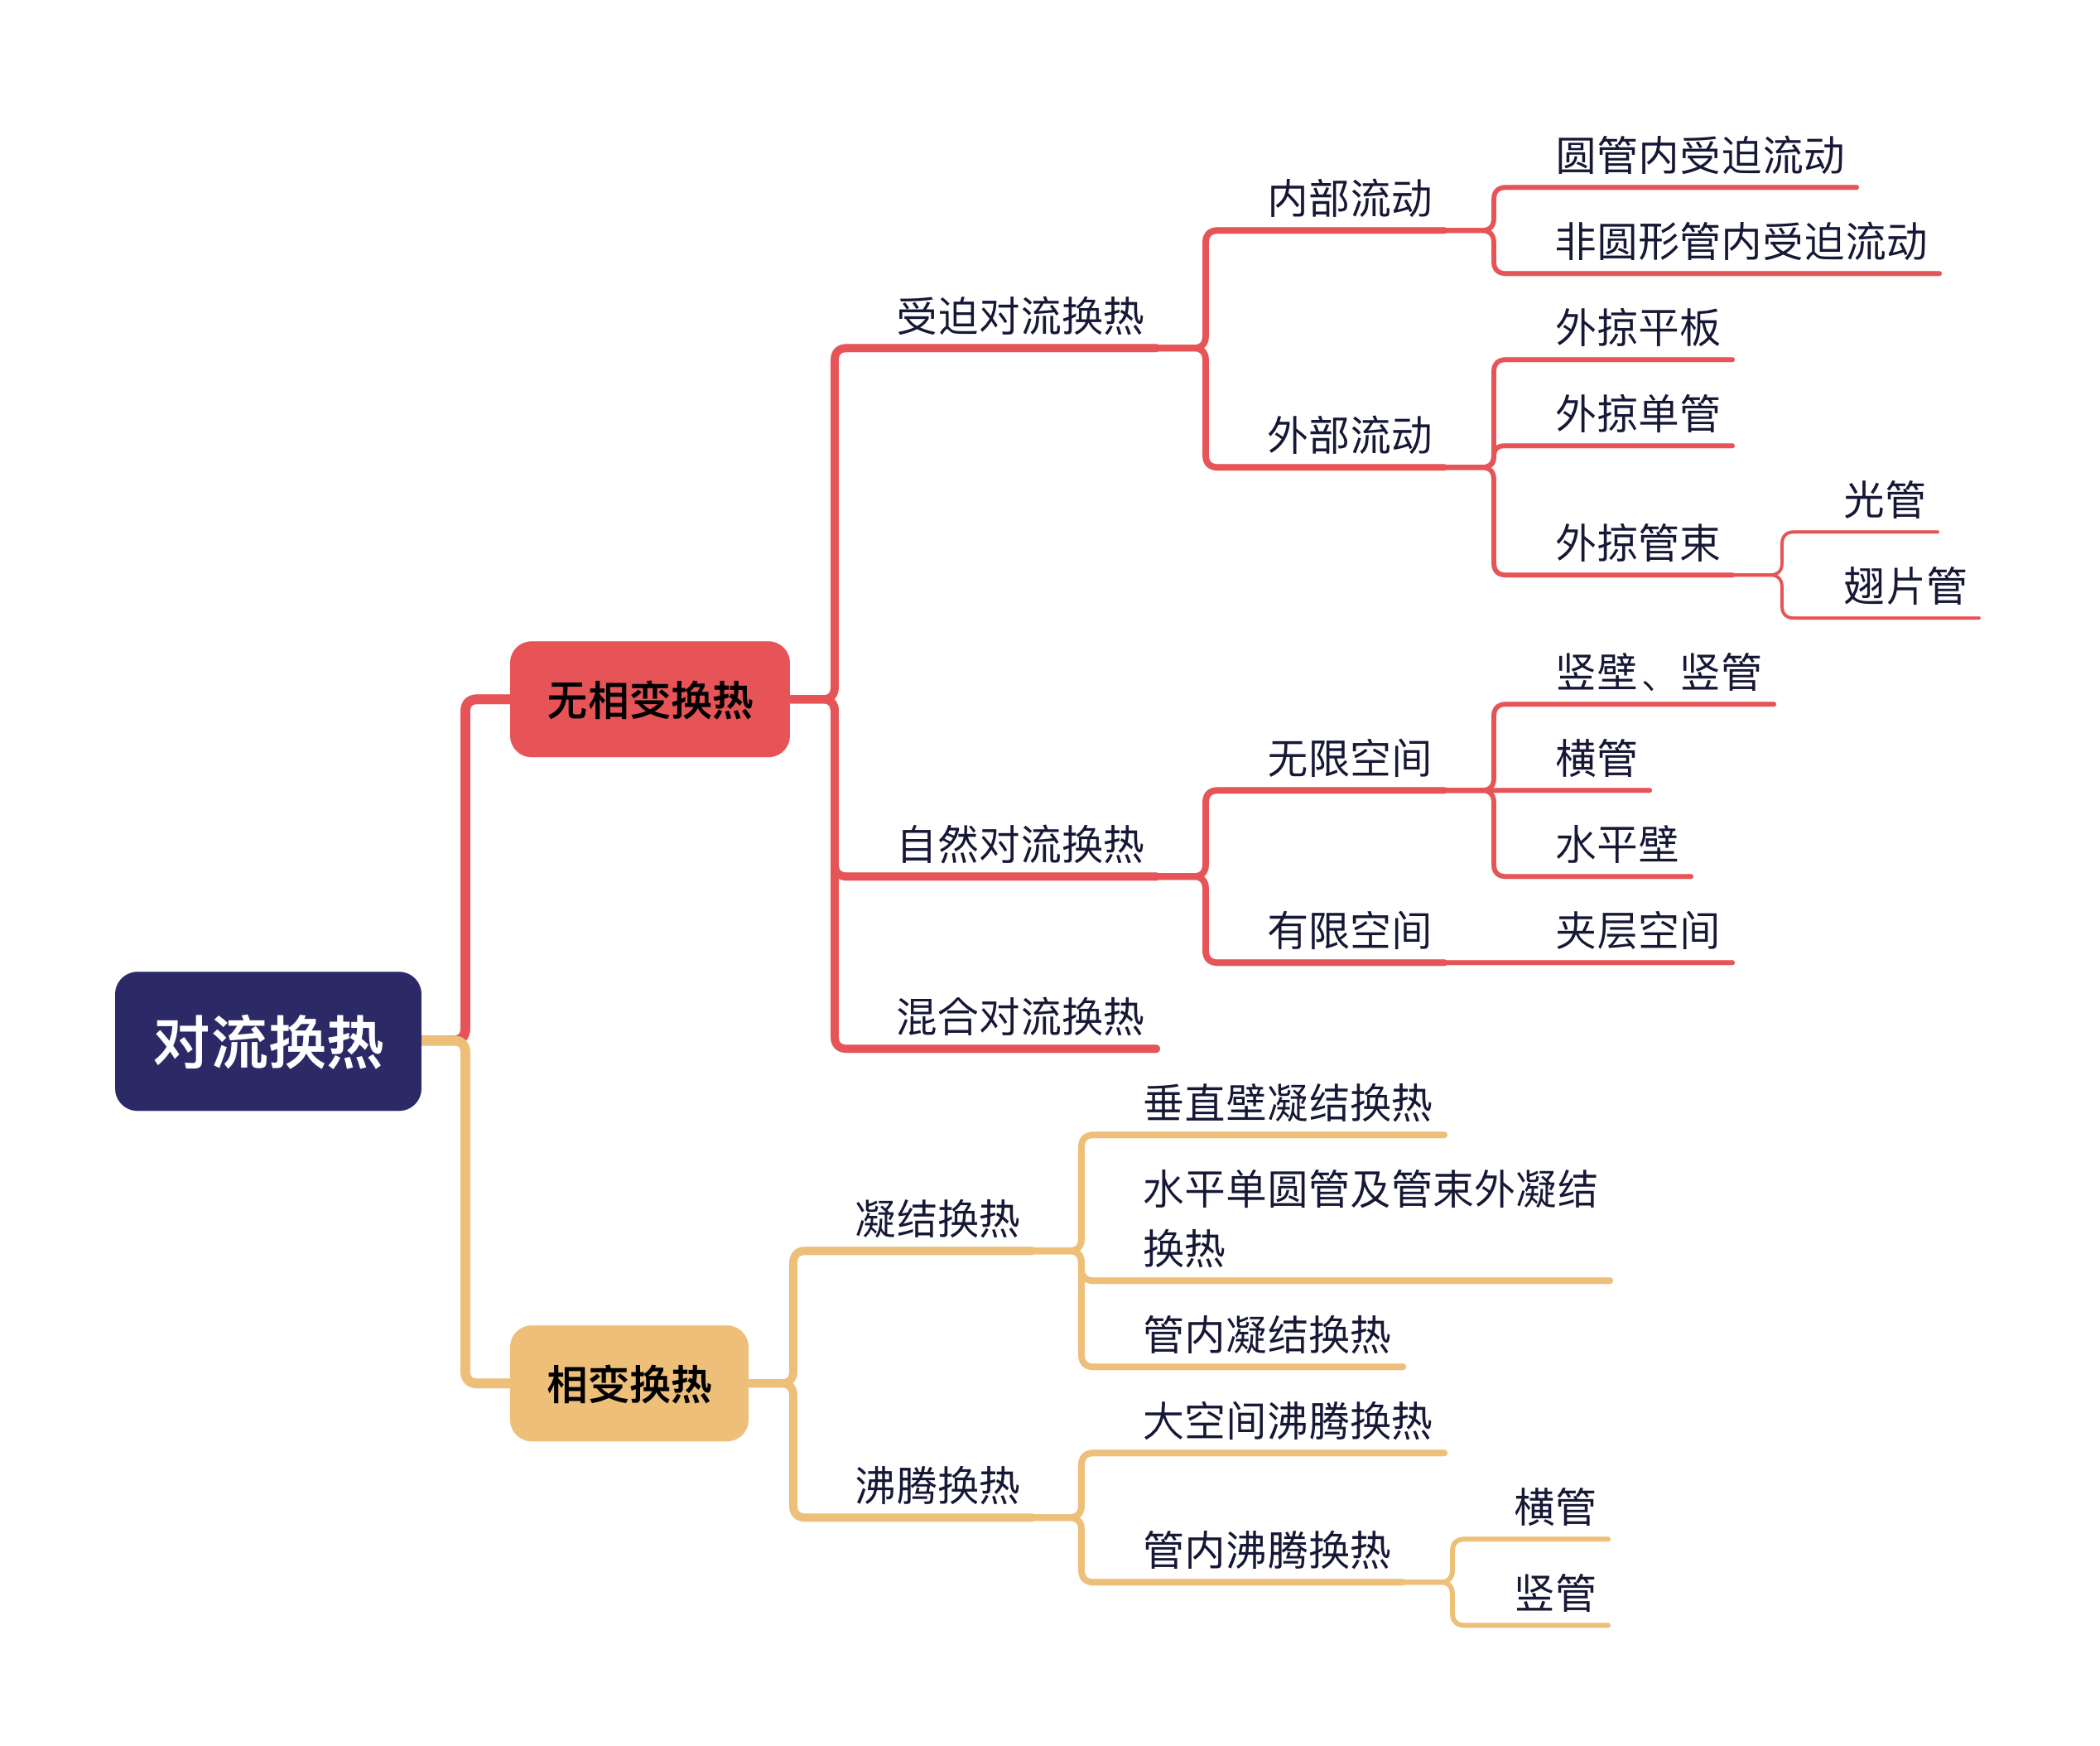
\includegraphics[width =.8\linewidth]{figures/7对流换热的分类.png}
%}

\pt{换热分类}：有无相变-流动起因-几何因素-流动状态\\
\pt{无相变换热}：受迫对流换热（内部流动：圆管、非圆形管；外部流动：外掠平板、外掠单管、外掠管束）；自然对流换热（无限空间：竖壁/竖管、横管、水平壁；有限空间：夹层空间）；混合对流换热。\\
\pt{相变换热}：凝结换热（垂直壁、水平单圆管及管束外、管内）；沸腾换热（大空间、管内）。

\pt{研究对流传热方法}分析法：采用数学分析求解，有指导意义。实验法：通过大量实验获得 $h$ 的计算式，是目前主要途径。比拟法：利用热量传递与动量传递的共性，建立 $h$ 与阻力系数之间关系，但限制较多。数值法：思想类似导热问题数值求解，发展迅速。

\pt{从温度场计算 $h$}：贴近壁面的薄层流体几乎不流动，热量传递主要靠导热。壁面局部热流密度：$q_{w,x}=-\lambda\left.\frac{\partial t}{\partial y}\right\vert_{y=0,x}$。换热热流密度：$q_{c,x}=h_x(t_{w,x}-t_{\infty})$。$q_{w,x}=q_{c,x}$，$h_x=-\lambda\frac{\left.\partial t/\partial y\right\vert_{y=0,x}}{t_{w,x}-t_{\infty}}$。

与导热第三类边界条件区别：导热问题中 $h$ 已知；这里 $h$ 是待求量。导热问题中 $\lambda$ 是固体导热系数；这里 $\lambda$ 是流体导热系数。导热问题中 $t$ 是固体温度；这里 $t$ 是流体温度。

\divider

%\subsection{对流问题的数学描述}

\pt{对流问题求解思路}流场由连续方程、运动方程描述。温度场由能量方程描述。求得温度场后，再由壁面温度梯度求 $h_x$。
\pt{简化假设}:二维问题。不可压缩、牛顿流体。常物性、无内热源。流速不高，忽略黏性耗散。不计流体与壁面之间的辐射换热。


\pt{能量稳态方程}

$\underbrace{\rho c_p\frac{\partial t}{\partial\tau}}_{\text{非稳态项}}+\underbrace{\rho c_p(u\frac{\partial t}{\partial x}+\nu\frac{\partial t}{\partial y})}_{\text{对流项}}=\underbrace{\lambda(\frac{\partial^2t}{\partial x^2}+\frac{\partial^2t}{\partial y^2})}_{\text{导热项}}$

$u,v$ 分别为 $x,y$ 方向的速度分量

\pt{物理含义}：对流传热温度场来自能量守恒与“导热 + 对流”的热量输运形式。对流传热中的微元体是固定空间内的开口系统，有流体流入与流出。总能量关系可写成 $\Phi=\partial U/\partial \tau+H_{\mathrm{out}}-H_{\mathrm{in}}$。 导热项：单位时间内由导热导入微元体的净热量：$\Phi=\lambda(\partial^2 t/\partial x^2+\partial^2 t/\partial y^2)\mathrm{d}x\mathrm{d}y$。热力学能增量：$\partial U/\partial \tau=\rho c_p(\partial t/\partial \tau)\mathrm{d}x\mathrm{d}y$。焓差项：不可压缩流体下，$H_{\mathrm{out}}-H_{\mathrm{in}}=\rho c_p(u\partial t/\partial x+v\partial t/\partial y)\mathrm{d}x\mathrm{d}y$。

当 $u=v=0$ 时，方程退化为纯导热方程

\pt{控制方程}：

\pt{能量微分方程}$\rho c_{p}\left(\frac{\partial t}{\partial\tau}+u\frac{\partial t}{\partial x}+\nu\frac{\partial t}{\partial y}\right)=\lambda\left(\frac{\partial^{2}t}{\partial x^{2}}+\frac{\partial^{2}t}{\partial y^{2}}\right)$
\pt{连续性方程} $\frac{\partial u}{\partial x}+\frac{\partial\nu}{\partial y}=0$
\pt{运动微分方程}$\rho\frac{\mathrm{D}u}{\mathrm{\tau}}=\vec{F}-\nabla \vec{p}+\mu\nabla^2u$

%$$
%    \left\{
%    \begin{aligned}
%         & \frac{\partial u}{\partial x}+\frac{\partial\nu}{\partial y}=0 \\&\rho(\frac{\partial u}{\partial\tau}+u\frac{\partial u}{\partial x}+\nu\frac{\partial u}{\partial y})=F_{x}-\frac{\partial p}{\partial x}+\mu(\frac{\partial^{2}u}{\partial x^{2}}+\frac{\partial^{2}u}{\partial y^{2}})\\&\rho(\frac{\partial\nu}{\partial\tau}+u\frac{\partial\nu}{\partial x}+\nu\frac{\partial\nu}{\partial y})=F_{y}-\frac{\partial p}{\partial y}+\mu(\frac{\partial^{2}\nu}{\partial x^{2}}+\frac{\partial^{2}\nu}{\partial y^{2}})\\&\rho c_{p}\left(\frac{\partial t}{\partial\tau}+u\frac{\partial t}{\partial x}+\nu\frac{\partial t}{\partial y}\right)=\lambda\left(\frac{\partial^{2}t}{\partial x^{2}}+\frac{\partial^{2}t}{\partial y^{2}}\right)\\&h_{x}=-\frac{\lambda}{t_{w,x}-t_{\infty}}\left.\frac{\partial t}{\partial y}\right\vert_{y=0,x}
%    \end{aligned}
%    \right.
%$$

对二维、不可压、常物性、牛顿流体、无内热源问题，未知量为 $u$、$v$、$t$、$p$、$h_x$，无第三类边界条件，因为 $h_x$ 为未知量。方程非线性，运动方程与能量方程耦合，因此引入边界层概念来简化控制方程组。

\divider

%\subsection{边界层型对流传热问题的数学描述}

\pt{流动边界层}定义：流体流过固体壁面时，由于黏性作用，在壁面附近形成速度剧烈变化的薄层，称为流动边界层或速度边界层。速度边界层厚度：定义为速度达到主流速度 $99\%$ 的位置，即 $u_{\delta}=0.99u_{\infty}$。

\pt{流动边界层特点}：$\delta$ 比壁面尺度 $l$ 小一个数量级以上，$\delta\ll l$。边界层内也有层流和湍流之分；外掠平板临界雷诺数 $\mathrm{Re}_c=5\times 10^5$。边界层内沿厚度方向速度梯度很大，边界层外速度梯度近似为 $0$。$\delta$ 沿流动方向逐渐增加。因边界层很薄，可近似认为同一截面上边界层内压强等于外边界压强，即 $y$ 方向压强近似相等。边界层内黏性力与惯性力同一数量级。

\pt{引入速度边界层的意义}：流动区域可分为主流区和边界层区。主流区可近似看作理想流体流动。只在边界层区考虑黏性作用。

\pt{温度边界层}：对流传热时，壁面附近温度发生剧烈变化的薄层称为温度边界层或热边界层。

\pt{热边界层厚度}：可用 $(T-T_w)\vert_{\delta_t}=0.99(T_{\infty}-T_w)$ 表征。热边界层厚度 $\delta_t$ 也满足 $\delta_t\ll l$。

\pt{温度边界层意义}：温度场也可分为主流区和边界层区；主流区温度变化可看作近似为零；只需重点确定边界层区内流体温度分布。

\pt{层流与湍流热边界层}：湍流边界层贴壁处温度梯度明显大于层流。因 $h_x$ 与壁面温度梯度有关，湍流换热强于层流。

\pt{普朗特数}：$\mathrm{Pr}=\nu/a$。 $\nu$ 表征动量扩散能力，越大则黏性影响传递越远，流动边界层越厚。$a$ 表征热扩散能力，越大则温度扰动传递越快，热边界层越厚。$\delta/\delta_t\approx \mathrm{Pr}^{1/3}$，$\mathrm{Pr}>1$ ，$\delta>\delta_t$；$\mathrm{Pr}<1$ ，$\delta_t>\delta$。（通常）

流体按 $\mathrm{Pr}$ 分类：高普朗特数流体：如油类，约 $10^2\sim 10^3$。中等普朗特数流体：约 $0.7\sim 10$，如气体 $0.7\sim 1.0$，水 $0.9\sim 10$。低普朗特数流体：如液态金属，约 $0.01$。

简化后的二维、稳态边界层对流传热微分方程组：\\
\pt{连续方程}：$\frac{\partial u}{\partial x}+\frac{\partial\nu}{\partial y}=0$。\\
\pt{$x$ 方向动量方程}：$u\frac{\partial u}{\partial x}+\nu\frac{\partial u}{\partial y}=-\frac{1}{\rho}\frac{dp}{dx}+\upsilon\frac{\partial^{2}u}{\partial y^{2}}$。\\
\pt{能量方程}：$u\frac{\partial t}{\partial x}+\nu\frac{\partial t}{\partial y}=a\frac{\partial^{2}t}{\partial y^{2}}$。\\
\pt{局部换热系数}：$h_{x}=-\frac{\lambda}{t_{w,x}-t_{\infty}}\frac{\partial t}{\partial y}|_{y=0,x}$。\\
$y=0$，$u=0$，$v=0$，$t=t_w$；$y\to\infty$，$u=u_{\infty}$，$t=t_{\infty}$。

未知参数 $u.v.t.h_x$ 适用条件：二维、稳态、不可压缩常物性、牛顿流体、无内热源、重力场可忽略、主流方向二阶导数可忽略。若流场产生旋涡，如湍流，则需用完整控制方程组描述。

\divider

%\subsection{外掠等温平板对流传热的解}

恒定壁温时流体纵掠平板换热，且流态为层流。假设恒定壁温；流体纵向掠过平板；二维、稳态、无内热源、重力场可忽略；主流场匀速、匀温；对外掠等温平板，主流压强梯度为 $-\mathrm{d}p/\mathrm{d}x=0$。

\pt{解的形式}：局部换热系数 $h_x=0.332\frac{\lambda}{x}\left(\frac{u_\infty x}{\nu}\right)^{0.5}\left(\frac{\nu}{a}\right)^{1/3}=0.332\frac{\lambda}{x}\mathrm{Re}^{0.5}\mathrm{Pr}^{1/3}$，局部努塞尔数 $\mathrm{Nu}_x=0.332\mathrm{Re}_x^{0.5}\mathrm{Pr}^{1/3}$，局部雷诺数 $\mathrm{Re}_x=\frac{u_\infty x}{\nu}$，离平板前缘 $x$ 处边界层厚度 $\frac{\delta}{x}=\frac{5.0}{\sqrt{\mathrm{Re}_x}}$，$\delta = 5.0\sqrt{\frac{\nu x}{u_\infty}}$，范宁局部摩擦系数 $c_f =\frac{t_w}{0.5\rho {u_\infty}^2}=\frac{0.664}{\sqrt{\mathrm{Re}_x}}$，流动边界层与热边界层之比 $\delta/\delta_t\cong \mathrm{Pr}^{1/3}$，适用条件 $\mathrm{Re}<5\times 10^5$（以上所有公式）

$\mathrm{Nu}$ 数与 $\mathrm{Bi}$ 数的区别：局部努塞尔数：$\mathrm{Nu}_x=h_xx/\lambda$；毕渥数：$\mathrm{Bi}=hl/\lambda$；$\lambda$ 不同：$\mathrm{Nu}$ 中的 $\lambda$ 是流体导热系数；$\mathrm{Bi}$ 中的 $\lambda$ 是导热物体内部的导热系数；$h$ 的角色不同：$\mathrm{Nu}$ 中的 $h$ 通常是待求的对流换热系数；$\mathrm{Bi}$ 中的 $h$ 常作为已知边界换热条件；物理含义不同：$\mathrm{Nu}$ 表示壁面上流体的无量纲温度梯度；$\mathrm{Bi}$ 表示导热热阻与对流换热热阻的相对大小。

长度为 $l$ 的等温平板平均换热系数：$h_l=\frac{\int_{0}^{l} h_x \, \mathrm{d}x}{l}$；层流平均换热系数：$h_l=0.664(\frac{\lambda}{l})\mathrm{Re}_l^{0.5}\mathrm{Pr}^{1/3}$；平均努塞尔数：$\mathrm{Nu}_l=0.664\mathrm{Re}_l^{0.5}\mathrm{Pr}^{1/3}$；$\mathrm{Nu}$、$\mathrm{Re}$ 中的特征长度为平板长度 $l$；物性参数定性温度取边界层平均温度：$t_m=(t_\infty+t_w)/2$。

\pt{比拟理论概念}：利用两个物理现象控制方程的类似性，通过测定其中一种现象的规律，获得另一现象的基本关系。对湍流换热，利用湍流中动量传递与热量传递机理类似，借助较易测定的湍流阻力系数推求湍流换热系数或 $\mathrm{Nu}$ 数。雷诺比拟：通过建立 $\mathrm{Nu}$ 与湍流阻力系数 $c_f$ 的关系，由 $c_f$ 求湍流对流换热近似解 $\mathrm{Nu}_x=c_f\mathrm{Re}_x/2$。平板湍流边界层阻力系数实验式：$c_f=0.0592\mathrm{Re}_x^{-1/5}$，适用 $\mathrm{Re}_x\le 10^7$。推得：$\mathrm{Nu}_x=0.0296\mathrm{Re}_x^{4/5}$，这是雷诺比拟结果，成立前提为 $\mathrm{Pr}=1$。用于一般流体时写成：$\mathrm{Nu}_x=0.0296\mathrm{Re}_x^{4/5}\mathrm{Pr}^{1/3}$

长平板 $l>x_c$ 时的分段处理：$x<x_c$：层流区，$\mathrm{Nu}_x=0.332\mathrm{Re}_x^{1/2}\mathrm{Pr}^{1/3}$；$x>x_c$：湍流区，$\mathrm{Nu}_x=0.0296\mathrm{Re}_x^{4/5}\mathrm{Pr}^{1/3}$。积分后平均努塞尔数：$\mathrm{Nu}_m=[0.664\mathrm{Re}_c^{1/2}+0.037(\mathrm{Re}_l^{4/5}-\mathrm{Re}_c^{4/5})]\mathrm{Pr}^{1/3}$。

\divider

%\subsection{相似原理与量纲分析}

对流换热研究方法：分析法，比拟法，基于相似理论的实验方法，数值计算方法。
需要解决的 Problem：对流传热实验变量多，实验中应测哪些量，是否所有物理量都测；对流传热实验数据如何整理，整理成什么样的函数关系；对流传热实验结果如何推广，实物实验无法开展时怎么办。

相似原理的基本内容：相似原理研究相似物理现象之间的关系。相似的物理现象：两个同类物理现象，如果在相应时刻、相应地点上，与现象有关的物理量一一对应成比例，则称两现象彼此相似。同类现象：由相同形式和内容的微分方程式描述，包括控制方程和单值性条件方程。注意区分“相似”与“类比/比拟”。对稳态对流换热，相似意味着换热面几何形状、温度场、速度场、物性场等相似。对非稳态问题，还要求相应时刻各物理量空间分布相似。

相似现象的特性：只有同类现象才能谈相似；彼此相似的现象，其有关物理量场分别相似；此相似的现象，其同名特征数，也称准则数，必定相等：两个相似的对流传热现象，其 $\mathrm{Nu}$ 数必定相等。

圆管内单相强制对流换热问题：$h=f(u,d,\lambda,\mu,\rho,c_p)$。
量纲分析目标：把有量纲变量关系化为无量纲准则关系。
上述问题有 $n=7$ 个物理量，涉及 $r=4$ 个基本量纲：时间 $T$、长度 $L$、质量 $M$、温度 $\Theta$。
所以可得到 $n-r=3$ 个无量纲准则数。
选 $u$、$d$、$\lambda$、$\mu$ 为基本物理量，其余 $h$、$\rho$、$c_p$ 与基本物理量组成 $\pi$ 方程。
得到：
$\pi_1=hd/\lambda=\mathrm{Nu}$;
$\pi_2=\rho ud/\mu=ud/\nu=\mathrm{Re}$;
$\pi_3=\mu c_p/\lambda=\nu/a=\mathrm{Pr}$。
因而强制对流关系可写成：$\mathrm{Nu}=f(\mathrm{Re},\mathrm{Pr})$。
自然对流换热：$\mathrm{Nu}=f(\mathrm{Gr},\mathrm{Pr})$。
混合对流换热：$\mathrm{Nu}=f(\mathrm{Re},\mathrm{Gr},\mathrm{Pr})$。
对流传热实验中，只需测量无量纲准则数所包含的物理量。研究其关系

应用相似原理可以减少实验次数，并得到有一定通用性的结果。应以已定特征数为参数安排实验。常用整理形式为幂函数形式：$\mathrm{Nu}=C\mathrm{Re}^n$。$\mathrm{Nu}=C\mathrm{Re}^n\mathrm{Pr}^m$。$\mathrm{Nu}=C\mathrm{Gr}^n\mathrm{Pr}^m$。$C$、$n$、$m$ 由实验数据确定，可用作图法或最小二乘法。这类无量纲准则数间关系式称为准则方程、特征数方程或实验关联式。\pt{管内强制湍流、流体被加热}时可整理得 $\mathrm{Nu}=0.023\mathrm{Re}^{0.8}\mathrm{Pr}^{0.4}$。

\pt{实验关联式的推广条件}：
判别物理现象相似的条件：
同名已定特征数相等。
单值性条件相似。
单值性条件包括：初始条件、边界条件、几何条件、物理条件。
已定特征数：由所研究物理现象中已知量组成的特征数。
只要对流现象满足相似条件，实验关联式就可以推广。
实物实验无法开展时，可以由满足相似条件的模型实验代替。
不能严格满足完全相似时，至少应保证对现象起决定作用的关键特征数相等。
使用准则方程时必须明确适用范围。
特征长度、特征流速、定性温度的选取方式必须与建立准则方程时一致。

常见\pt{相似准则数及物理意义}：
努塞尔数：$\mathrm{Nu}=hl/\lambda$，表示流体壁面处法向无量纲过余温度梯度。
雷诺数：$\mathrm{Re}=ul/\nu$，表示惯性力与黏性力的相对大小。
普朗特数：$\mathrm{Pr}=\nu/a$，表示动量扩散能力与热量扩散能力的相对大小。
格拉晓夫数：$\mathrm{Gr}=g\alpha_V\Delta t l^3/\nu^2$，表示浮升力与黏性力的相对大小。

\divider

%\subsection{内部强制对流传热实验关系式}

\pt{管槽内强制流动与传热的特点}

外部流动中边界层一般不受限制；内部流动中边界层会受到另一侧固体壁面的限制，可能发生边界层干扰或汇合。

\pt{管内流态判别}：层流临界雷诺数 $\mathrm{Re}_c=2300$；$2300<\mathrm{Re}<10000$ 为过渡区；$\mathrm{Re}>10000$ 为旺盛湍流区。管内存在入口段，边界层由零开始发展并最终汇合，入口段内传热强度由高逐渐减弱。

入口段长度估算：层流 $\ell_e/d\approx0.05\mathrm{Re}\mathrm{Pr}$；湍流 $\ell_e/d\approx60$。管内换热边界条件主要有两类：恒定热流密度、恒定壁温。特征速度一般取截面平均流速，课件给出 $u_m=\frac{\int_{A_c}\rho u,\mathrm{d}A}{\rho A_c}$。定性温度多取截面上流体平均温度，$t_f=\frac{\int_{A_c}c_p\rho tu\,\mathrm{d}A}{\int_{A_c}c_p\rho u\,\mathrm{d}A}$；工程中常取进出口截面平均温度 $t_f=(t'_f+t''_f)/2$。

牛顿冷却公式：$\Phi=hA\Delta t_m$。恒热流时，平均温差可取 $\Delta t_m=t_w-t_f$。恒壁温时，局部温差沿管长变化，应按热平衡式 $hA\Delta t_m=q_m c_p(t''_f-t'_f)$，并用对数平均温差 $\Delta t_m=\frac{t''_f-t'_f}{\ln((t_w-t'_f)/(t_w-t''_f))}$。

\pt{管内湍流 Dittus-Boelter 公式} $\mathrm{Nu}_f=0.023\mathrm{Re}_f^{0.8}\mathrm{Pr}_f^n$；流体被加热时 $n=0.4$，被冷却时 $n=0.3$。适用范围：$\mathrm{Re}=10^4\sim1.2\times10^5$，$\mathrm{Pr}=0.7\sim120$，$\ell/d\ge60$，光滑管湍流充分发展段。
中等温差限制：气体 $\Delta t\le50^\circ\mathrm{C}$，水 $\Delta t\le20\sim30^\circ\mathrm{C}$，油 $\Delta t\le10^\circ\mathrm{C}$；这里 $\Delta t=t_w-t_f$，不是进出口温差。
不适用于液态金属，因为液态金属 $\mathrm{Pr}\sim10^{-2}$。
入口段修正：若 $\ell/d<60$，引入 $c_l=1+(d/\ell)^{0.7}$。
弯管或螺旋管修正：二次流会破坏热边界层、强化传热；课件给出气体 $c_r=1+1.77d/R$，液体 $c_r=1+10.3(d/R)^3$。
大温差修正：气体被加热 $c_t=(T_f/T_w)^{0.5}$，气体被冷却 $c_t=1$；液体被加热 $c_t=(\mu_f/\mu_w)^{0.11}$，液体被冷却 $c_t=(\mu_f/\mu_w)^{0.25}$。
修正后公式为 $\mathrm{Nu}_f=0.023\mathrm{Re}_f^{0.8}\mathrm{Pr}_f^n c_t c_l c_r$。

\pt{管内湍流的 Gnielinski 公式}  \\ $\mathrm{Nu}_f=\frac{(f/8)(\mathrm{Re}_f-1000)\mathrm{Pr}_f}{1+12.7(f/8)^{1/2}(\mathrm{Pr}_f^{2/3}-1)}[1+(d/\ell)^{2/3}]c_t$。
Darcy 阻力系数为 $f=(1.82\lg\mathrm{Re}-1.64)^{-2}$。
适用范围：光滑管道湍流过渡区与充分发展段，$\mathrm{Re}=10^4\sim1.2\times10^5$，$\mathrm{Pr}=0.7\sim120$，$\ell/d\ge60$
物性修正：气体 $c_t=(T_f/T_w)^{0.45}$，且 $T_f/T_w=0.5\sim1.5$；液体 $c_t=(\mathrm{Pr}_f/\mathrm{Pr}_w)^{0.11}$，且 $\mathrm{Pr}_f/\mathrm{Pr}_w=0.05\sim20$。

D-B 公式形式简单；Gnielinski 公式精度更高，要求较高时优先使用


\pt{管内层流的 Sieder-Tate 公式}

管内层流充分发展换热中，热边界条件影响显著；充分发展段的 $\mathrm{Nu}$ 与 $\mathrm{Re}$ 无关。
工程换热设备中，层流常处于入口段范围，因此使用 Sieder-Tate 公式：$\mathrm{Nu}_f=1.86(\frac{\mathrm{Re}_f\mathrm{Pr}_f}{\ell/d})^{1/3}(\frac{\mu_f}{\mu_w})^{0.14}$。
适用条件：$\mathrm{Re}<2300$，均匀壁温，入口段层流，且温差影响已修正。$\mu_f/\mu_w=0.0044\sim9.75$，$\mathrm{Pr}_f=0.48\sim16700$， $\left(\frac{\mathbf{Re}_f\mathbf{Pr}_f}{l/d}\right)^{1/3}\left(\frac{\mu_f}{\mu_w}\right)^{0.14}\geq2$

\divider

%\subsection{外部强制对流传热实验关联式}

\pt{外掠等温平板}：层流 $\mathrm{Nu}_x=0.332\mathrm{Re}_x^{1/2}\mathrm{Pr}^{1/3}$，湍流 $\mathrm{Nu}_x=0.0296\mathrm{Re}_x^{4/5}\mathrm{Pr}^{1/3}$。平板计算注意：局部特征尺度取 $x$，平均换热时取板长 $\ell$；定性温度取 $t_m=(t_\infty+t_w)/2$；特征速度取来流速度 $u_\infty$。

\pt{横掠单管平均换热关联式}采用分段幂次式 $\mathrm{Nu}=C\mathrm{Re}^n\mathrm{Pr}^{1/3}$。
横掠单管三大特征量：定性温度 $t_f=(t_w+t_\infty)/2$；特征长度为管外径 $d$；特征速度为来流速度 $u_\infty$。
横掠单管适用范围：气体和液体均适用；$t_\infty=15.5\sim980^\circ\mathrm{C}$，$t_w=21\sim1046^\circ\mathrm{C}$，$\mathrm{Re}=0.4\sim4\times10^5$；计算时需按 $\mathrm{Re}$ 分段取 $C,n$。

\pt{纵掠单管}可视作长 $\ell$、宽 $\pi d$ 的外掠平板处理；层流和湍流仍可套用外掠平板局部关联式。$\mathrm{Nu}_x=0.332\mathrm{Re}_x^{1/2}\cdot \mathrm{Pr}^{1/3}$，$\mathrm{Re}<5\times10^5$，层流；$\mathrm{Nu}_x=0.0296\mathrm{Re}_x^{4/5}\mathrm{Pr}^{1/3}$

\pt{外掠球体}关联式为 $\mathrm{Nu}=2+(0.4\mathrm{Re}^{1/2}+0.06\mathrm{Re}^{2/3})\mathrm{Pr}^{0.4}(\mu_\infty/\mu_w)^{1/4}$。定性温度取来流温度，特征速度取来流速度，特征长度取球直径；适用范围为 $\mathrm{Pr}=0.71\sim380$，$\mathrm{Re}=3.5\sim7.6\times10^6$。

\pt{横掠管束}中，管间相互影响明显；叉排扰动强、换热强、阻力大；顺排扰动小、换热弱、阻力小且易清洗。
管束后排会受前排影响，冲刷方向也会影响换热。
\pt{茹卡乌斯卡斯公式 Zhukauskas}写作 $\mathrm{Nu}_f=C\mathrm{Re}_{f,\max}^m\mathrm{Pr}_f^n(\mathrm{Pr}_f/\mathrm{Pr}_w)^k(s_1/s_2)^p\varepsilon_n$。
管束计算中，定性温度取进出口流体平均温度 $t_f=(t'_f+t''_f)/2$，特征长度取管外径 $d$，特征速度取最窄截面平均流速。
适用条件：管排总数 $\ge16$；小于 16 时要修正；管距参数 $s_1,s_2$ 已含在公式中；适用 $\mathrm{Pr}=0.6\sim500$，$\mathrm{Re}=1\sim2\times10^6$。

\divider

%\section{自然对流实验关联式}

自然对流传热是由温度场不均匀引起密度不均匀，并在重力作用下产生浮升力而形成的流动与传热现象。
自然对流的流动与传热不可分割；它不依靠泵或风机等外力推动。
不均匀温度场不一定引起自然对流：若热流体在上、冷流体在下，可能形成稳定分层；若热流体在下、冷流体在上，则更容易形成不稳定环流。
自然对流通常传热较弱，常成为主要热阻，但优点是经济、安全、安静。
自然对流总换热量常需同时考虑与周围气体的自然对流和与周围表面的辐射传热，二者量级可能相当。
热竖壁自然对流边界层中，壁面处 $y\to0$ 有 $u=0,T=T_w$；远离壁面 $y\to\infty$ 有 $u=0,T=T_\infty$；速度在边界层内部有最大值。
自然对流也分层流和湍流；层流时局部表面传热系数随高度增加而减小，过渡时增加，旺盛湍流时局部表面传热系数近似为常量。
自然对流流态判别主要用\pt{格拉晓夫数} $\mathrm{Gr}$。
自然对流按空间分为大空间和有限空间；大空间指边界层在发展过程中不受干扰，有限空间指空间大小会影响传热效果。
课件给出大空间判据示意：若 $a/H>0.28$、$b/H>0.01$，可按大空间处理。

\pt{自然对流控制方程与特征数}

局部表面传热系数可由壁面温度梯度写作 $h_x=-\frac{\lambda}{t_{w,x}-t_\infty}(\frac{\partial t}{\partial y})\vert_{y=0,x}$。
对竖直平板上空气被加热的边界层，可忽略 $x$ 方向二阶导数项和 $y$ 方向动量方程，得到边界层型方程。
浮升力来源可写作 $\frac{g}{\rho}(\rho_\infty-\rho)=g\alpha_V\theta$，即由“温压”驱动。
格拉晓夫数为 $\mathrm{Gr}=\frac{g\alpha_V\Delta t l^3}{\nu^2}$，表示浮升力与黏性力之比。
自然对流中，能量方程还引入 $\mathrm{Pr}$，因此 $\mathrm{Nu}=f(\mathrm{Gr},\mathrm{Pr})$。
瑞利数为 $\mathrm{Ra}=\mathrm{Gr}\mathrm{Pr}$，常将自然对流关联式写成 $\mathrm{Nu}=C(\mathrm{Gr}\mathrm{Pr})^n=C\mathrm{Ra}^n$。

\pt{大空间自然对流}

大空间自然对流平均努塞尔数关联式：$\mathrm{Nu}=C(\mathrm{Gr}\mathrm{Pr})^n=C\mathrm{Ra}^n$。
特征温度取边界层平均温度 $t_m=(t_w+t_\infty)/2$。
特征长度：竖平板和竖圆柱取表面高度 $l$，横圆柱取外径 $d$。
非均匀壁温情形也可近似套用均匀壁温关联式，取平均壁温计算。
气体的体膨胀系数可按理想气体取 $\alpha_V=1/T$，液体的 $\alpha_V$ 需查物性手册。
一般层流时 $n=1/4$，湍流时 $n=1/3$。
课件例题 1 比较 $l/d=10$ 的金属柱体水平或垂直放置冷却：在两种情形均为层流且忽略端面散热时，计算得 $h_l/h_d=0.69$，所以从自然对流冷却角度看，水平放置散热更强。

\pt{有限空间对流}

典型有限空间包括竖封闭夹层和水平封闭夹层。
有限空间中，夹层厚度 $\delta$ 对流动开展有重要影响；冷热壁面温差是流动动力。
有限空间常用 $\delta$ 作为特征长度，取 $\mathrm{Nu}_\delta=h\delta/\lambda$，$\mathrm{Gr}_\delta=\frac{g\alpha_V\delta^3(t_{w1}-t_{w2})}{\nu^2}$，$t_m=(t_{w1}+t_{w2})/2$。
当 $\mathrm{Gr}_\delta$ 很小时，封闭空气夹层近似为纯导热：竖夹层 $\mathrm{Gr}_\delta\le2860$，水平夹层 $\mathrm{Gr}_\delta\le2430$。
封闭空气夹层总传热量等于自然对流换热和辐射换热之和。
竖封闭夹层关联式为 $\mathrm{Nu}_\delta=C(\mathrm{Gr}_\delta\mathrm{Pr})^n(H/\delta)^{-1/9}$。
竖封闭夹层层流：$C=0.197,n=1/4$；湍流：$C=0.073,n=1/3$。
水平封闭夹层关联式为 $\mathrm{Nu}_\delta=C(\mathrm{Gr}_\delta\mathrm{Pr})^n$，课件标注适用于 $H\gg\delta$。
水平封闭夹层层流：$C=0.212,n=1/4$；湍流：$C=0.061,n=1/3$。
水平夹层是否发生自然对流取决于热面位置：热面在上、冷面在下时流体稳定，按纯导热；热面在下、冷面在上时容易发生自然对流。
课件例题 2 中，水平封闭空气夹层 $\delta=14,\mathrm{mm}$，上下壁温 $90^\circ\mathrm{C}$ 和 $30^\circ\mathrm{C}$；热面在上时纯导热，$q=124,\mathrm{W/m^2}$；热面在下时按自然对流计算，$q=260,\mathrm{W/m^2}$。

\divider

%\subsection{相变对流传热基础}

\pt{相变传热}

相变对流传热包括凝结与沸腾传热。
工程应用背景：
空调、冰箱中的冷凝器和蒸发器；
蒸汽发生器；
锅炉炉膛水冷壁。
相变换热特点：
有潜热释放或吸收，单位质量相变时传热量大；
影响因素多，常比单相对流更复杂。

\pt{凝结传热}

凝结定义：蒸汽与低于其饱和温度的壁面接触时形成液体的过程，通常条件是 $t_w<t_s$。
凝结分类：
膜状凝结：浸润性液体沿整个壁面形成液膜，并在重力作用下流动；
珠状凝结：非浸润性液体在壁面形成许多小液珠；
凝结热阻：
蒸汽与冷壁面之间的液体层面积越大、越厚，热阻越大；
液膜是膜状凝结的主要传热阻力来源。
珠状凝结的实现方式：
改变凝结蒸气特性，例如在蒸气中加入油类；
改变凝结表面特性，例如表面改性处理、涂层。
凝结传热系数：
珠状凝结传热系数高于膜状凝结，可记作 $h_{\mathrm{珠}}>h_{\mathrm{膜}}$。
珠状凝结难以长期保持，工程中大多数凝结换热属于膜状凝结。
凝结换热设备设计通常以膜状凝结为依据。

\pt{膜状凝结}

膜状凝结影响因素：
不凝结气体：增加传递阻力，降低蒸气凝结分压力，减小凝结驱动力。
管子排数及管束排列方式：顺排、叉排、辐向排列都会影响凝结液排出和液膜厚度。
管内冷凝：蒸汽流速低时可能出现上下分层，蒸汽流速高时可能出现环状流。
蒸气流速与流动方向：流速较高时，蒸气流对液膜表面产生明显黏滞应力。
蒸气过热度。
液膜过冷度及温度分布非线性。
膜状凝结强化目标：尽量减薄液膜厚度。
膜状凝结强化技术：
减薄液膜厚度，例如微肋管、强化凝结换热表面；
及时排液，例如沟槽管、泄流板、排液圈。
%延伸：膜状凝结强化的本质是降低液膜导热热阻，可从 $R_{\mathrm{cond}}\sim \delta/\lambda$ 理解：液膜厚度 $\delta$ 越小，热阻越小。

\pt{沸腾传热}

液体汽化有两种方式：
蒸发 $\mathrm{evaporation}$；
沸腾 $\mathrm{boiling}$。
沸腾定义：工质内部形成大量气泡，并由液态转换到气态的一种剧烈汽化过程。
沸腾分类：
按主体液体温度：过冷沸腾、饱和沸腾；
过冷沸腾：流体主体温度低于相应压力下的饱和温度。
按流动条件：大容器沸腾，也称池沸腾；强制对流沸腾。
大容器沸腾：加热壁面沉浸在具有自由表面的液体中发生的沸腾。
大容器饱和沸腾曲线分区：
自然对流区：$\Delta t<4^\circ\mathrm{C}$，温差较小，主要靠自然对流传热。
核态沸腾区：$4^\circ\mathrm{C}<\Delta t<35^\circ\mathrm{C}$，气泡在加热表面形成并脱离，传热效率显著提高；包括孤立汽泡区和汽块区。
过渡沸腾区：$35^\circ\mathrm{C}<\Delta t<200^\circ\mathrm{C}$，气泡部分覆盖加热表面，传热不稳定。
稳定膜态沸腾区：加热面被蒸汽膜覆盖，传热效率急剧下降。
曲线中的 $q_{\max}$ 为临界热流密度，也与烧毁点、DNB 转折有关；$q_{\min}$ 为最小热流密度。
沸腾换热强的原因：
气泡经历产生、成长、脱离过程。
气泡运动会扰动热边界层，增强近壁流体混合。
气化核心：
产生气泡的点称为气化核心。
壁面凹缝、裂穴最容易成为气化核心。

\pt{沸腾影响因素}

不凝结气体：
与膜状凝结不同，液体中的不凝结气体会使沸腾换热得到某种程度的强化。
过冷度：
液体平均温度小于饱和温度 $t_s$ 时发生过冷沸腾。
在核态沸腾起始阶段，自然对流占主导地位。
自然对流 $h$ 近似正比于 $\Delta t^{0.25}$，过冷度会强化传热。
液位高度：
存在临界液位。
液位低于一定高度时，表面传热系数会明显随液位降低而升高。
液位高于该高度时，沸腾换热表面传热系数与液位高度基本无关。
重力加速度：
在 $0.1$ 到 $100\times 9.8\ \mathrm{m/s^2}$ 范围内，$g$ 对核态沸腾换热规律没有明显影响。
$g$ 对自然对流换热有影响。
管内沸腾：
属于管内强制对流沸腾问题。
需要关注流动类型、换热类型、表面传热系数。

\pt{强化沸腾}

强化沸腾传热原则：增加汽化核心。
强化方法：
物理化学手段：烧结、钎焊、火焰喷涂、电离沉积等；
机械加工方法：制造粗糙表面、微结构或强化表面；
典型强化表面包括三维微肋管等。
延伸：
强化沸腾并不是简单提高壁温；壁温过高可能进入过渡沸腾或膜态沸腾，反而导致传热恶化甚至烧毁。

\pt{热管}

热管工作原理：
热端吸热，工质蒸发；
蒸汽在压差作用下流向冷端；
冷端放热，蒸汽凝结；
凝结液通过毛细结构或重力回流到热端，形成循环。
热管工作场景：
课件示例为笔记本电脑中芯片与散热器之间的热管冷却。
热管利用相变潜热传递热量，因此等效导热能力很强。

\divider
\end{cheatsheet}
\end{document}
